
\def\chapterillustration{./abertura-estatistica1}%Photo by Hoach Le Dinh on Unsplash, https://unsplash.com/photos/c8TWWQ5ZnUw?utm_source=unsplash&utm_medium=referral&utm_content=creditCopyText 
\def\chapterwhat{Especificidade do pensamento estatístico a partir de problemas. Conceitos: população e amostra, parâmetro e estimador. Variáveis estatísticas e suas classificações. Organização dos dados em tabelas de frequências. Representações gráficas adequadas para os diferentes tipos de variáveis. Noções básicas de amostragem.}
\def\chapterbecause{A Estatística está presente no mundo contemporâneo e chega aos cidadãos em todos os
meios de comunicação. Diariamente somos confrontados com informações estatísticas
sobre temas como Economia, Educação, Esportes, Saúde, Meio-Ambiente, entre outros.
Tais informações orientam decisões em nossas vidas pessoais e permitem-nos exercer
nossas responsabilidades como cidadãos. Um conhecimento básico de Estatística é
fundamental na formação do cidadão para que este possa, de forma competente, apreciar
e criticar argumentos baseados em dados.} 
\chapter{A Natureza da Estatística}
\label{\detokenize{PE103:a-natureza-da-estatistica}}\label{\detokenize{PE103::doc}}


\explore{a natureza da Estatística}
\label{\detokenize{PE103-0:explorando-compreendendo-a-natureza-da-estatistica}}\label{\detokenize{PE103-0::doc}}\label{\detokenize{PE103-0:cap-a-natureza-da-estatistica}}
Vivemos cercados de incertezas. A todo momento somos bombardeados por informações sobre pequisas científicas comprovando (estatisticamente) que tal substância causa uma patologia, ou sobre pesquisas de opinião, índices de pobreza, características sobre o envelhecimento da população, e outros temas de natureza incerta. Num mundo assim, é importante ter espírito crítico para informações sujeitas à incerteza a fim de poder interpretá-las e, quando necessário, poder escolher, entre diferentes opções, aquela que parece melhor diante da incerteza.  Nesse sentido, a Estatística é uma disciplina fundamental para todos os estudantes e, certamente, com grande responsabilidade para a formação crítica do cidadão, pois ela é usada nas mais variadas áreas do conhecimento tais como: Medicina, Economia, Política, Direito, Psicologia, Engenharia, Educação, entre outras.

Mas afinal o que é Estatística?
\begin{description}
\item[{Estatística\index{Estatística|textbf}}] \leavevmode\phantomsection\label{\detokenize{PE103-0:term-estatistica}}
Arte e ciência de coletar, analisar, apresentar e interpretar dados, para que se tomem decisões sob incerteza.
\end{description}

\begin{task}{Escolha do melhor fornecedor - Tomada de decisão}
\phantomsection\label{\detokenize{PE103-0:ativ-1-escolha-do-melhor-fornecedor}}

\emph{Controle de Qualidade na Produção de Parafusos (Inspirada em ROSSMAN and CHANCE, 1998).}


Uma indústria precisa comprar parafusos de diâmetro 15 mm cuja variação aceitável é 15,0 mm ``mais ou menos'' 0,2 mm. Há quatro empresas, A, B, C e D, fornecedoras desses parafusos, que são vendidos em caixas com 60 unidades. Para decidir de qual fornecedor passará a comprar os parafusos, a empresa resolveu comprar e analisar uma caixa de cada um dos fornecedores. Os diâmetros das peças foram medidos com instrumento de alta precisão e os valores obtidos estão representados nos gráficos a seguir, em que cada círculo representa um parafuso posicionado sobre a abscissa correspondente à medida do seu diâmetro, medido em precisão de 0,02 mm.
\phantomsection\label{\detokenize{PE103-0:fig-parafusos}}


\begin{center}
\begin{tikzpicture}[x = 200, y=5, scale=1.2]

   \draw [help lines, lightgray, xstep=0.02,   ystep=1,xshift=-0.6] (14.383,0) grid (15.625,15) ;
   \draw [eixos] (14.37,0) -- (15.65,0);
   \foreach \x in {0,...,12}{
   \newcommand \y {\pgfmathparse{14.4+0.1* \x}\pgfmathprintnumber{\pgfmathresult}}
      \coordinate (A\x) at ($(14.4,0)+(0.1*\x,0)$);
      \draw ($(A\x)+(0,2pt)$) -- ($(A\x)-(0,2pt)$);
      \node [below] at ($(A\x)-(0,0.5ex)$) {\small \y} ;
   }
   \node[left] at (15.6,16) {Fornecedor A};
   \foreach \x/\y in {14.42/1,14.44/8,14.46/9,14.48/10,14.50/13,14.52/7,14.54/8,14.56/3,14.58/1}{
      \foreach \i in {1,...,\y}{
         \filldraw[color=primario] (\x,\i) circle (1.5pt);
      }}
\end{tikzpicture}
   
\begin{tikzpicture}
\begin{scope}[x = 200, y=5, scale=1.2]

   \draw [help lines, lightgray, xstep=0.02,   ystep=1,xshift=-0.6] (14.383,0) grid (15.625,15) ;
   \draw [eixos] (14.37,0) -- (15.65,0);
   \foreach \x in {0,...,12}{
   \newcommand \y {\pgfmathparse{14.4+0.1*  \x}\pgfmathprintnumber{\pgfmathresult}}
      \coordinate (A\x) at ($(14.4,0)+(0.1*\x,0)$);
      \draw ($(A\x)+(0,2pt)$) -- ($(A\x)-(0,2pt)$);
      \node [below] at ($(A\x)-(0,0.5ex)$) {\small \y} ;
   }
   \node[left] at (15.6,16) {Fornecedor B};
   \foreach \x/\y in {14.6/1,14.82/1,14.84/1,14.86/1,14.88/3,14.9/3,14.92/3,14.94/3,14.96/2,14.98/6,15/10,15.02/4,15.04/5,15.06/3,15.08/2,15.1/6,15.12/2,15.18/3,15.24/1}{
      \foreach \i in {1,...,\y}{
         \filldraw[color=primario] (\x,\i) circle (1.5pt);
      }
   }
   \end{scope}
\end{tikzpicture}
   
\begin{tikzpicture}
\begin{scope}[x = 200, y=5, scale=1.2]

   \draw [help lines, lightgray, xstep=0.02,   ystep=1,xshift=-0.6] (14.383,0) grid (15.625,15) ;
   \draw [eixos] (14.37,0) -- (15.65,0);
   \foreach \x in {0,...,12}{
   \newcommand \y {\pgfmathparse{14.4+0.1*  \x}\pgfmathprintnumber{\pgfmathresult}}
      \coordinate (A\x) at ($(14.4,0)+(0.1*\x,0)$);
      \draw ($(A\x)+(0,2pt)$) -- ($(A\x)-(0,2pt)$);
      \node [below] at ($(A\x)-(0,0.5ex)$) {\small \y} ;
   }
   \node[left] at (15.6,16) {Fornecedor C};
   \foreach \x/\y in {14.48/1,14.52/1,14.54/1,14.62/2,14.66 /2,14.7/2,14.72/1,14.78/2,14.8/2,14.84/2,14.88/2,14.9 /2,14.92/4,14.98/3,15/5,15.02/4,15.04/1,15.08/3,15.12 /3,15.16/4,15.18/1,15.2/2,15.22/1,15.3/1,15.32/1,15.38 /1,15.44/2,15.46/1,15.48/2,15.6/1}{
      \foreach \i in {1,...,\y}{
         \filldraw[color=primario] (\x,\i) circle (1.5pt);
      }
   }
   \end{scope}
\end{tikzpicture}
   
\begin{tikzpicture}
\begin{scope}[x = 200, y=5, scale=1.2]

   \draw [help lines, lightgray, xstep=0.02,    ystep=1,xshift=-0.6] (14.383,0) grid (15.625,15) ;
   \draw [eixos] (14.37,0) -- (15.65,0);
   \foreach \x in {0,...,12}{
   \newcommand \y {\pgfmathparse{14.4+0.1*  \x}\pgfmathprintnumber{\pgfmathresult}}
      \coordinate (A\x) at ($(14.4,0)+(0.1*\x,0)$);
      \draw ($(A\x)+(0,2pt)$) -- ($(A\x)-(0,2pt)$);
      \node [below] at ($(A\x)-(0,0.5ex)$) {\small \y} ;
   }
   \node[left] at (15.6,16) {Fornecedor D};
   \foreach \x/\y in {14.46/1,14.48/2,14.54/1,14.58/1,14.62/3,14.64/5,14.68/6,14.7/4,14.72/2,14.74/9,14.76/1,14.78/3,14.8/2,14.82/2,14.88/3,14.9/2,14.92/2,14.94/4,14.96/2,15/1,15.02/1,15.08/1,15.12/1}{
      \foreach \i in {1,...,\y}{
         \filldraw[color=primario] (\x,\i) circle (1.5pt);
      }
   }
\end{scope}
\end{tikzpicture}

\end{center}


\begin{enumerate}
\item {} 
Que informações foram usadas para a construção desses gráficos?

\item {} 
Quantos parafusos da caixa do fornecedor A atendem a especificação do comprador?

\item {} 
Para cada fornecedor, identifique a medida do diâmetro de maior \index{frequência}frequência.

\item {} 
Considerando cada um dos fornecedores, identifique o menor e o maior diâmetros observados.

\item {} 
Com base na sua resposta anterior, identifique os fornecedores cujos diâmetros dos parafusos observados variaram nos intervalos de menor \index{amplitude}amplitude e de maior amplitude.


\begin{description}
\item[{Amplitude\index{Amplitude|textbf}}] \leavevmode\phantomsection\label{\detokenize{PE103-0:term-amplitude}}
Em Estatística, a amplitude é definida como a diferença entre o maior e o menor valores observados.

\end{description}

\item De qual fornecedor você classifica o comportamento dos diâmetros dos parafusos como o de maior    \index{dispersão}dispersão? E o de menor dispersão?
\begin{description}
\item[{Dispersão\index{Dispersão|textbf}}] \leavevmode\phantomsection\label{\detokenize{PE103-0:term-dispersao}}
Segundo o dicionário Aurélio, dispersão significa (1) ato ou efeito de dispersar; (2) separação (de pessoas ou coisas) para diferentes partes.  Em Estatística, existem diferentes medidas de dispersão, dentre as quais, a amplitude.

\end{description}

\item Com base nesses dados, a(s) caixa(s) de qual(is)  fornecedor(es) apresenta(m) pelo menos um parafuso dentro das especificações do comprador?

\item Supondo que, para cada fornecedor, os comportamentos dos diâmetros dos parafusos sejam similares para as outras caixas, que fornecedor, com base nas especificações do comprador, você recomendaria ao comprador? Por quê?

\item Todos os parafusos da caixa do fornecedor escolhido no item anterior seriam aproveitados?
\end{enumerate}

\end{task}


\begin{reflection}

\begin{itemize}
\item Comente a estratégia usada para a obtenção dos dados dos fornecedores: as medidas obtidas refletem o comportamento das medidas de todos os parafusos produzidos pelo fornecedor? Seria razoável medir todos os parafusos fabricados por um fornecedor?

\item Que procedimento você usaria para confirmar a sua escolha inicial?

\item Em Controle de Qualidade, área de aplicação da Estatística na Indústria, é muito comum realizar comparações de diferentes produtos para fazer uma escolha ou verificar se os mesmos atendem às especificações apresentadas. Proponha um problema desse tipo com algum produto e indique a estratégia a ser usada e que medidas deveriam ser observadas.

\end{itemize}
\end{reflection}

\phantomsection\label{\detokenize{PE103-0:ativ-2-comparacao-de-medicamentos}}
\begin{task}{ Comparação de medicamentos}

Deseja-se comparar três medicamentos, X, Y e Z, no tratamento da dor de cabeça. Para isso 60 pacientes com perfis similares foram separados aleatoriamente em três grupos de 20 cada. Para cada grupo,  será ministrado um dos medicamentos e observado o tempo de cura da dor de cabeça (em minutos). No quadro a seguir estão dispostos os dados obtidos.
\phantomsection\label{\detokenize{PE103-0:tabela-medicamentos}}

\begin{savenotes}\sphinxattablestart
\centering
\begin{tabulary}{\linewidth}[t]{|T|T|T|T|T|T|T|T|T|T|T|T|T|T|T|T|T|T|T|T|T|T|}
\hline
\sphinxstylethead{\sphinxstyletheadfamily 
medicamento
\unskip}\relax &\sphinxstartmulticolumn{20}%
\begin{varwidth}[t]{\sphinxcolwidth{20}{22}}
\sphinxstylethead{\sphinxstyletheadfamily tempo em minutos
\unskip}\relax \par
\vskip-\baselineskip\vbox{\hbox{\strut}}\end{varwidth}%
\sphinxstopmulticolumn
&\sphinxstylethead{\sphinxstyletheadfamily 
soma
\unskip}\relax \\
\hline
X
&
7
&
8
&
8
&
9
&
9
&
9
&
9
&
10
&
10
&
10
&
10
&
10
&
10
&
11
&
11
&
11
&
11
&
12
&
12
&
13
&
200
\\
\hline
Y
&
7
&
8
&
9
&
9
&
10
&
10
&
11
&
11
&
11
&
12
&
12
&
12
&
13
&
13
&
14
&
14
&
15
&
15
&
16
&
18
&
240
\\
\hline
Z
&
11
&
11
&
11
&
11
&
11
&
12
&
12
&
12
&
12
&
12
&
12
&
12
&
12
&
12
&
12
&
13
&
13
&
13
&
13
&
13
&
240
\\
\hline
\end{tabulary}
\par
\sphinxattableend\end{savenotes}
\begin{enumerate}
\item {} 
Organize as informações apresentadas no quadro acima em diagramas de pontos. Utilize uma folha de papel quadriculada, usando a mesma escala.

\item {} 
A partir dos diagramas construídos, identifique o grupo que apresentou maior dispersão dos tempos de cura com base na amplitude.

\item {} 
Determine os tempos médios de cura da dor de cabeça para cada substância.

\item {} 
A partir dos diagramas construídos e das médias calculadas, responda:
\begin{enumerate}
\item Entre X e Y, qual medicamento você escolheria? Por quê?
\item Entre X e Z, qual medicamento você escolheria? Por quê?
\item Entre Y e Z, qual medicamento você escolheria? Por quê?
\item A partir dos dados disponíveis, é possível garantir que algum medicamento é melhor que os outros? Por quê?
\end{enumerate}
\end{enumerate}
\end{task}

\begin{research}

Em casa, procure algum remédio e leia a sua bula. Em seguida, identifique informações que você considera como resultantes de estudos que envolvam Estatística e anote-as em seu caderno.

\end{research}


\phantomsection\label{\detokenize{PE103-0:ativ-3-pesquisa-ibge-pnad}}
\begin{task}{ Pesquisa sobre a prática de esportes e atividade física}

\emph{Fonte: IBGE, Suplemento da PNAD/2015}

A Pesquisa Nacional por \index{Amostra}Amostra de Domicílios (PNAD), realizada pelo \href{https://www.ibge.gov.br/estatisticas-novoportal/sociais/populacao/9127-pesquisa-nacional-por-amostra-de-domicilios.html}{IBGE}, obtém informações anuais sobre características demográficas e socioeconômicas da população, como sexo, idade, educação, trabalho e rendimento, e características dos domicílios. Com periodicidade variável, a PNAD obtém informações sobre migração, fecundidade, entre outras, tendo os domicílios como unidade de coleta da informação. Temas específicos abrangendo aspectos demográficos, sociais e econômicos também são investigados.

Um aspecto fundamental da Estatística praticado nessa pesquisa é a forma na qual a \index{amostra}amostra, subconjunto da \index{população}população, é selecionada. Essa seleção é cuidadosamente planejada de modo que seja adequado estender os resultados obtidos na amostra para a população.

Para que os resultados de uma amostra possam ser estendidos para a população, é necessário planejar com cuidado como a amostra será selecionada, pois o critério de seleção da amostra depende da estrutura da população. Por exemplo, para saber se o feijão cozinhando na panela está bem temperado, basta provar uma pequena colherada. Por quê?  Partimos do pressuposto de que todos os ingredientes foram bem misturados e, assim, a mistura é homogênea.

Quando dispomos de dados provenientes de um subconjunto da população sempre podemos descrever os dados nos restringindo apenas ao subconjunto. Se quisermos estender nossas conclusões para a população, será necessário o uso de outras tecnologias que permitam calcular as incertezas associadas a essas extensões.

Na PNAD 2015 foi realizada a investigação de um tema específico chamado ``Suplemento de Práticas de Esporte e Atividade Física'' no qual foram investigadas as pessoas moradoras de 15 anos ou mais de idade, \textbf{em seu tempo livre}, no período de referência de 365 dias, com o objetivo de quantificar aquelas que praticaram algum esporte ou atividade física no período considerado bem como a sua percepção quanto a isso. As informações levantadas nessa pesquisa foram obtidas por meio de um questionário no qual se perguntou:
\begin{itemize}
\item {} 
Se a pessoa moradora havia praticado esporte, e em caso afirmativo, a respectiva modalidade.

\item {} 
Independente da resposta anterior, também se perguntou se a pessoa praticava alguma atividade física que não considerava como esporte, informando, em caso positivo, também a modalidade.

\item {} 
Outras informações levantadas nessa pesquisa foram: motivação para a prática da atividade física, local onde é praticada a atividade, frequência na qual a atividade é praticada, duração da atividade; e a participação em competições.

\item {} 
Também foram levantadas informações sobre as pessoas que responderam que não praticavam atividade física. Perguntou-se o motivo de não o fazerem e se haviam praticado anteriormente, caso em que se perguntou a modalidade praticada, a idade em que parou de praticar e a causa da interrupção.

\item {} 
Além dessas informações, a pesquisa investigou também a avaliação da população sobre a opção de o poder público investir no desenvolvimento de atividades físicas e esportivas ou em outra área (saúde, educação, etc.) na vizinhança de seu domicílio.

\end{itemize}
\begin{enumerate}
\item {} 
Liste pelo menos oito \index{variáveis}variáveis investigadas na PNAD e no ``Suplemento de Práticas de Esporte e Atividade Física'' da PNAD 2015, baseando-se no texto apresentado.

\item {} 
Das variáveis citadas no item anterior, quais delas apresentam respostas não numéricas?

\item {} 
Das variáveis citadas no item a), quais delas apresentam respostas numéricas?

\end{enumerate}

Cada uma das unidades investigadas em um estudo estatístico é denominada um \index{elemento}elemento.  Assim, cada parafuso investigado é um elemento na atividade ``Escolha do fornecedor''; cada paciente observado é um elemento na atividade ``Comparação de medicamentos''; e cada domicílio e seus residentes são elementos na atividade da PNAD.

Cada característica observada de um elemento é uma \index{variável}variável estatística. Assim, a medida do diâmetro do parafuso é uma variável na atividade ``Escolha do fornecedor'', o tempo de cura da dor de cabeça é uma variável na atividade ``Comparação de medicamentos'' e, na atividade da PNAD, estão presentes várias variáveis estatísticas de interesse do domicílio e de seus residentes tais como local, número de cômodos, número de residentes; sexo, idade e rendimento dos residentes, etc.
\end{task}

\phantomsection\label{\detokenize{PE103-0:ativ4-analise-de-infograficos}}
\begin{task}{ Análise de infográficos}

A seguir apresentaremos quatro \index{infográficos}infográficos, produzidos pelo IBGE (\href{https://vamoscontar.ibge.gov.br/atividades/ensino-medio/9801-pesquisando-a-pratica-de-esportes-e-atividades-fisicas-no-brasil.html}{vamoscontar.ibge.gov.br}) usando os dados do Suplemento Prática de Esporte e Atividade Física da PNAD 2015.

Um \index{infográfico}infográfico é uma apresentação de informações integradas em textos sintéticos com dados numéricos e elementos gráficos e visuais tais como fotografias, desenhos, diagramas estatísticos, gráficos, etc.

\begin{figure}[H]
\centering
\capstart

\noindent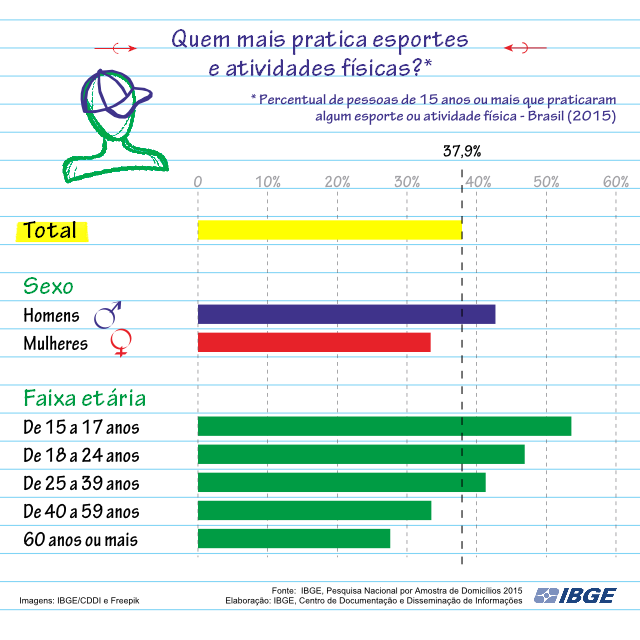
\includegraphics[width=300bp]{PNAD_2015_Esportes_01quem2.png}
\caption{PNAD - Infográfico 1}\label{\detokenize{PE103-0:fig-infografico-pnad-1}}\label{\detokenize{PE103-0:id1}}\end{figure}
\begin{enumerate}
\item {} 
Segundo a pesquisa, qual a porcentagem de pessoas de 15 anos ou mais que praticaram algum esporte ou atividade física no período de um ano?

\item {} 
O título genérico deste infográfico, a saber, ``Quem mais pratica esportes e atividades físicas? - Percentual de pessoas de 15 anos ou mais que praticaram algum esporte ou atividade física-Brasil (2015)'', diz respeito à população brasileira de 15 anos ou mais ou à amostra coletada?

\item {} 
Com base nas recomendações médicas sobre a prática de atividades físicas para se ter boa saúde, como você avalia o resultado obtido na pesquisa para a população brasileira de 15 anos ou mais?

\item {} 
Considerando homens e mulheres separadamente, percebe-se alguma diferença com relação à prática de atividades físicas? Em caso afirmativo, descreva a(s) diferença(s) observada(s).

\item {} 
Considerando as faixas etárias discriminadas no infográfico, percebe-se alguma diferença com relação à prática de atividades físicas? Em caso afirmativo, descreva a(s) diferença(s) observada(s).

\end{enumerate}

\begin{figure}[H]
\centering
\capstart

\noindent\includegraphics[width=300bp]{{PNAD_2015_Esportes_03instrrend2}.png}
\caption{PNAD - Infográfico 2}\label{\detokenize{PE103-0:fig-infografico-pnad-2}}\label{\detokenize{PE103-0:id2}}\end{figure}
\begin{enumerate}
\item {} 
Considerando os diferentes graus de instrução, percebe-se alguma diferença com relação à prática de atividades físicas? Em caso afirmativo, descreva a(s) diferença(s) observada(s).

\item {} 
Considerando as faixas de rendimento mensal per capita do domicílio, percebe-se alguma diferença com relação à prática de atividades físicas? Em caso afirmativo, descreva a(s) diferença(s) observada(s).

\end{enumerate}

\begin{figure}[H]
\centering
\capstart

\noindent\includegraphics[width=300bp]{{PNAD_2015_Esportes_04principais}.png}
\caption{PNAD - Infográfico 3}\label{\detokenize{PE103-0:fig-infografico-pnad-3}}\label{\detokenize{PE103-0:id3}}\end{figure}
\begin{enumerate}
\item {} 
Qual foi a variável estudada no gráfico acima?

\item {} 
A variável estudada tem respostas de que tipo: numéricas ou não-numéricas?

\item {} 
Qual foi a resposta que apresentou a maior frequência?

\item {} 
O que você acha que representa a resposta ``Outros Esportes''?

\end{enumerate}

\begin{figure}[H]
\centering
\capstart

\noindent\includegraphics[width=300bp]{{PNAD_2015_Esportes_05investimento}.png}
\caption{PNAD - Infográfico 4}\label{\detokenize{PE103-0:fig-infografico-pnad-4}}\label{\detokenize{PE103-0:id4}}\end{figure}
\begin{enumerate}
\item {} 
Qual a porcentagem de pessoas de 15 anos ou mais que concorda com que o poder público deva investir em atividades físicas ou desportivas?

\item {} 
Qual a opinião das pessoas de 15 anos ou mais que concordam que o poder público deve investir em atividades físicas ou esportivas com relação à prioridade de investimentos?

\item {} 
Entre as pessoas de 15 anos ou mais que não concordam que o poder público deve investir em atividades físicas ou esportivas, que área elas entendem como prioritária?

\item {} 
Podemos afirmar que 57,8\% das pessoas de 15 anos ou mais defendem que o poder público deve investir em Saúde?''

\end{enumerate}
\end{task}


\arrange{ }
\label{\detokenize{PE103-1:organizando-as-ideias}}\label{\detokenize{PE103-1::doc}}
Nas atividades anteriores foram trabalhados vários conceitos importantes da Estatística. Alguns desses conceitos serão apresentados a seguir.
\phantomsection\label{\detokenize{PE103-1:sub-conceitos-basicos}}
\textbf{Conceitos Básicos}

Em geral, a palavra população representa um conjunto de habitantes de um determinado lugar. No entanto, em Estatística, \index{população}população tem um sentido mais amplo e pode ser definida como o conjunto de todos os elementos com pelo menos uma característica em comum. Observe que é exatamente essa característica em comum que vai definir o universo (população) de uma pesquisa.

Assim, em Estatística, a população não precisa ser um conjunto de pessoas, pode ser o conjunto de parafusos fabricados por uma indústria, o conjunto de animais de certa espécie que vivem em uma região, todos os estudantes universitários de um país, etc.
\begin{description}
\item[{Amostra\index{Amostra|textbf}}] \leavevmode\phantomsection\label{\detokenize{PE103-1:term-amostra}}
é um subconjunto não-vazio da população.

\end{description}

Cada uma das unidades investigadas em um estudo estatístico é denominada um \index{elemento}elemento.  Assim, cada parafuso investigado é um elemento na atividade ``Escolha do fornecedor''; cada paciente observado é um elemento na atividade ``Comparação de medicamentos''; e cada domicílio e seus residentes são elementos na atividade da PNAD.

Cada característica observada de um elemento é uma \index{variável}variável estatística. Assim, a medida do diâmetro do parafuso é uma variável na atividade ``Escolha do fornecedor'', o tempo de cura da dor de cabeça é uma variável na atividade ``Comparação de medicamentos'' e, na atividade da PNAD, estão presentes várias variáveis estatísticas de interesse do domicílio e de seus residentes tais como local, número de cômodos, número de residentes; sexo, idade e rendimento dos residentes, etc.

Suponha que deseja-se investigar a opinião dos estudantes de um colégio quanto à modificação da lista de produtos vendidos na cantina para outros mais saudáveis, trocando refrigerantes por sucos naturais entre outros. Para isso, a direção da escola irá entrevistar cinco alunos sorteados de cada uma de suas 40 turmas. Nesse exemplo, a população corresponde a todos os estudantes deste colégio e, a amostra, aos 200 estudantes que foram entrevistados. Cada estudante entrevistado é um elemento e, a variável de interesse  é a opinião do estudante: ``a favor'' ou ``contra'' à mudança. Num estudo desse tipo, costuma-se registrar também outras variáveis como sexo, idade, ano de ensino, turno, etc.
\begin{description}
\item[{Parâmetro\index{Parâmetro|textbf}}] \leavevmode\phantomsection\label{\detokenize{PE103-1:term-parametro}}
característica numérica da população.

\end{description}
\begin{description}
\item[{Estimador\index{Estimador|textbf}}] \leavevmode\phantomsection\label{\detokenize{PE103-1:term-estimador}}
função que produz estimativas de parâmetros usando os dados da amostra.

\end{description}

Voltando ao exemplo anterior, sobre a modificação da lista de produtos da cantina, temos que o parâmetro corresponde à proporção dos estudantes desse colégio que são favoráveis à mudança (na maioria das vezes não acessível, a menos que se realize um censo). O estimador desse parâmetro corresponderá à proporção de estudantes favoráveis à mudança na amostra, que resultará numa estimativa do parâmetro.

As etapas da análise estatística podem ser divididas em duas estruturas básicas: \index{Estatística Descritiva}Estatística Descritiva e \index{Estatística Inferencial}Estatística Inferencial. A primeira corresponde a uma exploração das informações que podem ser retiradas dos dados amostrais de modo a reconhecer estruturas que possibilitem futuramente inferir sobre parâmetros de interesse. A segunda consiste em estabelecer modelos probabilísticos para que se possa fazer afirmações sobre a população com algum nível de confiança. Vide a caixa ``Para refletir'' a seguir.

Em resumo, a Estatística Descritiva é uma espécie de arqueologia dos dados observados e, a Estatística Inferencial, a indução das informações obtidas da amostra para características da população não observada em sua totalidade.

A PNAD faz uso da inferência estatística, pois ela investiga uma amostra de domicílios em algumas cidades brasileiras, mas propõe estimativas para as características da população brasileira.

Quando se realiza um \index{censo}censo - levantamento de dados de toda a população -, não existe a necessidade de fazer uma inferência estatística. No entanto, muitas vezes a realização de um censo é inviável, por várias razões como custo muito alto, tempo muito longo, entre outras.

\begin{reflection}
Proposições são elementos importantes na construção de toda a ciência. No que se refere à natureza da Estatística, em contraponto à natureza da Matemática, podemos destacar dois tipos de proposições.

Uma proposição é dita matemática se é possível classificá-la em \emph{verdadeira} ou \emph{falsa}, ainda que essa afirmação seja uma conjectura não provada. Assim, a proposição

\emph{``O quadrado de um número par é par.''}

é uma proposição matemática, pois sabemos que ela é verdadeira. Da mesma forma, a proposição

\emph{``O triângulo de lados 6, 4 e 3 é um triângulo retângulo.''}

é uma proposição matemática, pois sabemos que é falsa.

Por outro lado, uma proposição estatística é uma afirmação sobre a qual nunca teremos condição de afirmar se é \emph{verdadeira} ou \emph{falsa}, mas apenas aferir um nível de confiança para ela. A proposição
\begin{itemize}
\item {} 
``Uma moeda, que ao ser lançada 10 vezes, resulta em 10 coroas, não é uma moeda equilibrada.''*

\end{itemize}

é uma proposição estatística, pois existe a possibilidade de em 10 lançamentos de uma moeda equilibrada obtermos 10 coroas, embora isso seja pouco provável de ocorrer.

\textbf{Observação:} Uma moeda é dita ser equilibrada se as probabilidades de se obter cara e coroa são iguais. Caso contrário, a moeda é dita ser não-equilibrada.

Se lançarmos 100 vezes essa mesma moeda e obtivermos 8 caras, teremos mais evidências para aceitar a proposição de que não seja equilibrada, mas ainda assim não poderemos afirmar que a proposição seja verdadeira. Proposições desse tipo que envolvem um nível de confiança sobre sua veracidade são propsições de natureza estatística.
\end{reflection}
\phantomsection\label{\detokenize{PE103-1:sub-classificacao-de-variaveis}}
\textbf{Classificação de variáveis}

A classificação das variáveis estudadas é importante, pois as técnicas e procedimentos estatísticos de análise de dados dependem do tipo de variável investigado. Nesse sentido é importante reconhecer a natureza de cada variável investigada para posterior tratamento da informação obtida. Por exemplo, se estamos estudando a modalidade de atividades físicas praticadas pelos brasileiros de 15 anos ou mais, não faz sentido calcular média, pois  ela não assume valores numéricos.

Existem dois tipos principais de variáveis (qualitativas e quantitativas), que se subdividem, por sua vez, em duas categorias, conforme a figura 2.2.
\phantomsection\label{\detokenize{PE103-1:fig-classificacao-de-variaveis}}\begin{figure}[htp]\centering\begin{tikzpicture}
\tikzstyle{vecArrow} = [thick, decoration={markings , mark=at position
1 with {\arrow[semithick, fill=white]{triangle 60}}},
double distance=1.4pt, shorten >= 5.5pt,
preaction = {decorate,line width=1.4pt},
postaction = {draw,line width=1.4pt, white,shorten >= 4.5pt}]
\begin{scope}[x=15, y=10]

   \draw[rounded corners = 5pt, fill=primario] (-9,0) rectangle (-5,2);
   \node[color=white] at (-7,1) {nominal};
   \draw[rounded corners = 5pt, fill=primario] (-4.5,0) rectangle (-0.5,2);
   \node[color=white] at (-2.5,1) {ordinal};
   \draw[rounded corners = 5pt, fill=primario] (0.5,0) rectangle (4.5,2);
   \node[color=white] at (2.5,1) {discreta};
   \draw[rounded corners = 5pt, fill=primario] (5,0) rectangle (9,2);
   \node[color=white] at (7,1) {contí­nua};
   \draw[vecArrow] (-4.75,3.25) -- (-6,1.5);
   \draw[vecArrow] (-4.75,3.25) -- (-3.5,1.5);
   \draw[vecArrow] (4.75,3.25) -- (6,1.5);
   \draw[vecArrow] (4.75,3.25) -- (3.5,1.5);
   \draw[rounded corners = 5pt, fill=primario] (-9,3) rectangle (-0.5,5);
   \node[color=white] at (-4.75,4) {qualitativa};
   \draw[rounded corners = 5pt, fill=primario] (0.5,3) rectangle (9,5);
   \node[color=white] at (4.75,4) {quantitativa};
   \draw[vecArrow] (0,6.25) -- (-1.5,4.5);
   \draw[vecArrow] (0,6.25) -- (1.5,4.5);
   \draw[rounded corners = 5pt, fill=primario] (-9,6) rectangle (9,8);
   \node[color=white] at (0,7) {Variável};


\end{scope}
\end{tikzpicture}\caption{Classificação dos tipos de variáveis}\end{figure}\begin{description}
\item[{Variável qualitativa\index{Variável qualitativa|textbf}}] \leavevmode\phantomsection\label{\detokenize{PE103-1:term-variavel-qualitativa}}
Uma variável estatística é qualitativa se as possíveis respostas para ela são atributos não-numéricos. A maior parte das variáveis identificadas no ``Suplemento de Práticas de Esporte e Atividade Física'' da PNAD/2015, representa variáveis qualitativas.

\end{description}

Uma variável qualitativa é classificada em nominal ou ordinal.
\begin{description}
\item[{Variável qualitativa nominal\index{Variável qualitativa nominal|textbf}}] \leavevmode\phantomsection\label{\detokenize{PE103-1:term-variavel-qualitativa-nominal}}
Uma variável qualitativa é nominal quando não existe nenhuma ordenação natural das respostas associadas à variável. Exemplos de variáveis nominais: bairro de residência, tipo sanguíneo, modalidade de atividade física que pratica, etc.

\end{description}
\begin{description}
\item[{Variável qualitativa ordinal\index{Variável qualitativa ordinal|textbf}}] \leavevmode\phantomsection\label{\detokenize{PE103-1:term-variavel-qualitativa-ordinal}}
A variável qualitativa é ordinal quando é possível estabelecer uma relação de ordem entre as respostas associadas a ela. Por exemplo, nível de instrução da mãe com as respostas possíveis: Ensino Fundamental completo, Ensino Médio completo, Ensino Superior incompleto e Ensino Superior completo. Podemos perceber que quem tem Ensino Médio completo tem maior nível de instrução de quem tem Ensino Fundamental completo.

\end{description}
\begin{description}
\item[{Variável quantitativa\index{Variável quantitativa|textbf}}] \leavevmode\phantomsection\label{\detokenize{PE103-1:term-variavel-quantitativa}}
Uma variável é quantitativa se as respostas para ela são numéricas. Exemplos de variáveis quantitativas são idade, peso, altura, temperatura, número de irmãos, número de horas semanais dedicadas à prática de atividade física.

\end{description}

Uma variável quantitativa é classificada em discreta ou contínua.
\begin{description}
\item[{Variável quantitativa discreta\index{Variável quantitativa discreta|textbf}}] \leavevmode\phantomsection\label{\detokenize{PE103-1:term-variavel-quantitativa-discreta}}
As variáveis discretas resultam de uma contagem ou são variáveis cuja quantidade de valores possíveis é finita. Por exemplo, o número de atendimentos em um Pronto-Socorro nos finais de semana, o número de erros de impressão na página de um livro, número de irmãos, etc.

\end{description}
\begin{description}
\item[{Variável quantitativa contínua\index{Variável quantitativa contínua|textbf}}] \leavevmode\phantomsection\label{\detokenize{PE103-1:term-variavel-quantitativa-continua}}
As variáveis quantitativas contínuas em geral resultam de uma medição. Por exemplo, altura, peso, temperatura, etc.

\end{description}

\begin{observation}

Na análise dos infográficos vimos que uma variável quantitativa pode ser tratada como qualitativa, por exemplo, a idade trabalhada em faixas etárias torna-se uma variável qualitativa ordinal. No entanto, se consideramos a idade em anos completos temos uma variável quantitativa. Por outro lado, também podemos transformar uma variável qualitativa em quantitativa. Considere a variável ``prática de atividades físicas'' que tem como respostas ``Sim'' ou ``Não''. Esse tipo de variável com apenas duas respostas é chamado \index{variável binária}variável binária e tem uma representação numérica natural. Podemos atribuir o número 1 para a resposta ``Sim'' e o número 0 para a resposta ``Não''. Essa estratégia permite somar todas as respostas. Observe que a soma representará o número de pessoas na amostra que praticam atividade física e a ``média'' representará a proporção de pessoas na amostra que praticam atividade física.
\end{observation}

\textbf{Gráficos para Variáveis Qualitativas}

Nas análises dos infográficos, trabalhamos com alguns tipos de gráficos para representar a distribuição de frequências de variáveis qualitativas. No {\hyperref[\detokenize{PE103-0:fig-infografico-pnad-3}]{\sphinxcrossref{\DUrole{std,std-ref}{infográfico 3}}}}, tem-se um \index{gráfico de barras}gráfico de barras. Nesse gráfico, cada barra, de mesma largura, representa uma resposta e seu comprimento corresponde à \index{frequência}frequência na qual a resposta ocorre. Observe também que, nesse gráfico, se estivermos trabalhando com as porcentagens de cada resposta, a soma das porcentagens deve ser 100\%.

Em geral, se a variável for ordinal dispomos as respostas em ordem crescente. Se a variável é nominal, podemos dispor as respostas em ordem decrescente de frequência.

\begin{example}{Frequência absoluta e frequência relativa}

Numa turma de um colégio foram observados os tipos sanguíneos de seus 40 alunos. Verificou-se que 18 alunos têm sangue tipo ``O'', 12, tipo ``A'', 6, tipo ``AB'' e 4, tipo ``B''. Nesse exemplo, temos que as \index{frequência absoluta}frequências absolutas para os tipos sanguíneos ``O'', ``A'', ``AB'' e ``B'' foram, respectivamente, 18, 12, 6 e 4. Em geral, quando queremos comparar grupos diferentes, usamos a \index{frequência relativa}frequência relativa em vez da frequência absoluta. A frequência relativa é dada pela razão entre a frequência absoluta e o número total de observações. Nesse exemplo, temos que as frequências relativas para os tipos sanguíneos ``O'', ``A'', ``AB'' e ``B'' foram, respectivamente, 0,45; 0,30; 0,15 e 0,10. Observe que em termos percentuais as frequências relativas observadas equivalem a, respectivamente, 45\%, 30\%, 15\% e 10\%.
É comum resumir esse tipo de informação, usando uma tabela, informando as respostas da variável e suas frequências. Nesse exemplo a variável é tipo sanguíneo e sua classificação é qualitativa nominal, pois assume respostas não numéricas ``A'', ``B'', ``AB'' e ``O'', sem uma ordenação natural. Em geral dispomos os valores dessa variável em ordem decrescente de frequência.


\begin{savenotes}\sphinxattablestart
\centering
\begin{tabulary}{\linewidth}[t]{|T|T|T|T|}
\hline
\sphinxstylethead{\sphinxstyletheadfamily 
tipo
sanguíneo
\unskip}\relax &\sphinxstylethead{\sphinxstyletheadfamily 
frequência
absoluta
\unskip}\relax &\sphinxstylethead{\sphinxstyletheadfamily 
frequência
relativa
\unskip}\relax &\sphinxstylethead{\sphinxstyletheadfamily 
porcentagem
(\%)
\unskip}\relax \\
\hline
O
&
18
&
0,45
&
45
\\
\hline
A
&
12
&
0,30
&
30
\\
\hline
AB
&
6
&
0,15
&
15
\\
\hline
B
&
4
&
0,10
&
10
\\
\hline
total
&
40
&
1,00
&
100
\\
\hline
\end{tabulary}
\par
\sphinxattableend\end{savenotes}
\end{example}

Os gráficos apresentados nos {\hyperref[\detokenize{PE103-0:fig-infografico-pnad-1}]{\sphinxcrossref{\DUrole{std,std-ref}{infográfico 1}}}} e {\hyperref[\detokenize{PE103-0:fig-infografico-pnad-2}]{\sphinxcrossref{\DUrole{std,std-ref}{infográfico 2}}}} são gráficos de barras?

Esses gráficos usam barras para representar as frequências em subgrupos diferentes do conjunto observado. Mas eles não se encaixam na apresentação anterior. Verifique que se somarmos as porcentagens elas não resultarão em 100\%. De fato, são \index{gráficos de barras múltiplas}gráficos de barras múltiplas, úteis para comparar diferentes distribuições de frequências. Observe que, em cada um desses gráficos, a variável sob investigação é se a pessoa pratica ou não atividade física. No entanto, em vez de apresentar as porcentagens das respostas \emph{Sim} e \emph{Não} no universo de homens e no universo de mulheres, como a variável é binária, só foram apresentadas as porcentagens de \emph{Sim} em cada subgrupo, pois nesse caso, as correspondentes porcentagens de \emph{Não} são dadas pelo complementar em cada subgrupo considerado.

\begin{figure}[H]
\centering
\capstart

\noindent\includegraphics[width=400pt]{{barrasmultiplas_sexo}.png}
\caption{Detalhe legendado do \DUrole{xref,std,std-ref}{infográfico 1}}\label{\detokenize{PE103-1:fig-infografico-1-detalhe}}\label{\detokenize{PE103-1:id2}}\end{figure}

O mesmo ocorre quando analisamos os gráficos para faixa etária, grau de instrução e rendimento. Todos são gráficos de barras múltiplas que nos apoiaram em nossas análises sobre a associação entre a prática de atividades físicas e a outra variável (sexo, faixa etária, grau de instrução, rendimento).

No {\hyperref[\detokenize{PE103-0:fig-infografico-pnad-4}]{\sphinxcrossref{\DUrole{std,std-ref}{infográfico 4}}}}, temos um \index{gráfico de setores}gráfico de setores e dois \index{gráficos de retângulos}gráficos de retângulos. A ideia por trás desses gráficos é subdividir de maneira proporcional a figura maior em partes cujas áreas em relação à figura maior correspondam à frequência de cada resposta. Por exemplo, no gráfico de setores, subdividimos o círculo em setores de tal modo que a razão da área de cada setor em relação a área do círculo corresponde à frequência (ou porcentagem) da resposta que ele representa. Portanto a soma das frequências, quando apresentadas em porcentagens, tem que ser igual a 100$\%$.

No gráficos de retângulos essa mesma ideia é usada: o retângulo maior é subdividido em retângulos cujas áreas relativas correspondem às porcentagens das respostas que eles representam. Esses gráficos foram construídos para representar as respostas à pergunta ``Em quais áreas em que deve ocorrer investimento público?'' para quem respondeu \emph{Não} à pergunta ``O poder público deve investir em atividades físcas ou desportivas?'' e também para representar as respostas à pergunta ``Qual deve ser a prioridade nos investimentos?'' para quem respondeu ``Sim'' à pergunta ``O poder público deve investir em atividades físicas ou desportivas?''.

\begin{observation}

Quando estamos trabalhando com variáveis qualitativas usamos a escala da frequência (absoluta, relativa, porcentagem)  na construção de gráficos para representar a distribuição de frequências das respostas dadas à variável sob investigação. As representações gráficas mais comuns são gráficos de barras e gráficos de setores. Para comparações da mesma variável em grupos diferentes é comum usar o gráfico de barras múltiplas com frequências relativas ou porcentagens.
\end{observation}

\practice{ }
\label{\detokenize{PE103-2::doc}}\label{\detokenize{PE103-2:praticando}}\phantomsection\label{\detokenize{PE103-2:ativ-1-pratica-atividade-fisica-na-turma}}
\begin{task}{ Prática de atividade física na turma}


Deseja-se comparar os hábitos de atividade física em tempo livre dos alunos da turma com os dados obtidos da PNAD/2015. Para isso preencha o formulário de dados fornecido pelo professor. Construa tabelas e gráficos resumindo a informação obtida.
\end{task}
\phantomsection\label{\detokenize{PE103-2:ativ-classificacao-de-variaveis}}
\begin{task}{ Classificação de variáveis}

Suponha que cada uma das variáveis a seguir foi observada para todos os alunos de sua turma. Indique se cada uma delas é uma variável qualitativa ou quantitativa. Se for uma variável qualitativa, indique se ela é binária (apenas duas respostas possíveis) ou não.
\begin{enumerate}
\item {} 
altura (em metros)

\item {} 
peso (em quilos)

\item {} 
razão do peso sobre o quadrado da medida da altura

\item {} 
tempo de sono na noite anterior

\item {} 
se foi dormir na noite anterior antes ou depois da meia-noite

\item {} 
mês de nascimento

\item {} 
número de irmãos

\item {} 
nota obtida na última avaliação de Matemática

\item {} 
se tirou nota maior ou igual a 6,0 ou menor do que 6,0 na última avaliação de Matemática

\item {} 
distância da casa à escola

\item {} 
se o indivíduo possui cartão de crédito ou não

\item {} 
modo de locomoção para a escola

\end{enumerate}
\end{task}
\phantomsection\label{\detokenize{PE103-2:ativ-3-construcao-de-grafico-variavel-qualitativa}}
\begin{task}{ Construção de gráficos para variáveis qualitativas}

Considerando o {\hyperref[\detokenize{PE103-0:fig-infografico-pnad-4}]{\sphinxcrossref{\DUrole{std,std-ref}{infográfico 4}}}}, transforme o gráfico de setores em gráfico de retângulos e os gráficos de retângulos em gráficos de setores.
\end{task}

\phantomsection\label{\detokenize{PE103-2:ativ-4-analise-de-grafico}}
\begin{task}{ Análise de gráfico}

Observe o gráfico a seguir publicado em um jornal.
\begin{enumerate}
\item {} 
Como você classificaria esse gráfico?

\item {} 
Qual é a informação representada pelo comprimento da barra nesse gráfico?

\item {} 
Que tipo(s) de variável(is) ele está representando?

\item {} 
Construa um gráfico diferente para representar a mesma informação, marcando num plano Cartesiano os pontos (x,y) em que x corresponde ao tempo e y corresponde à inflação acumulada no domicílio, unindo os pontos consecutivos por segmentos. É possível perceber a partir desse gráfico algum tipo de comportamento no período observado?

\end{enumerate}
\phantomsection\label{\detokenize{PE103-2:linhaversusbarra}}\begin{figure}[htp]\centering\begin{tikzpicture}
\begin{scope}[x=20, y = 10]
\draw (0,0) -- (28,0);
\foreach \ye in {-5,5,10,15}{
\draw [help lines, lightgray] (0,\ye) -- (28,\ye);
}
\foreach \x/ \y/\z in {1/16.79/AGO,2/16.11/SET,3/14.85/OUT,4 /11.57/NOV,5/9.36/DEZ,6/6.47/JAN,7/4.34/FEV,8/3/MAR,9 /2.54/ABR,10/1.08/MAI,11/-0.56/JUN,12/-3.07/JUL,13/-5.19 /AGO}{
   \draw [fill=primario] (2*\x-0.5,0) rectangle  (2*\x+0.5,\y);
   \node at (2*\x,-8) {\z};
}
\node at (2,-9) {2016};
\node at (12,-9) {2017};
\node [right] at (0,21.5) {INFLAÇÃO DA ALIMENTAÇÃOO NO   DOMICÍLIO};
\node [right] at (0,20) {(acumulado em 12 meses, em   $\%$)};\\
\end{scope}
\end{tikzpicture}\caption{Inflação da alimentação acumulada nos últimos 12 meses (Fonte: IBGE)}\end{figure}\end{task}



\explore{estruturas de variáveis quantitativas}
\label{\detokenize{PE103-3:explorando-visualizando-estruturas-de-variaveis-quantitativas}}\label{\detokenize{PE103-3::doc}}\phantomsection\label{\detokenize{PE103-3:ativ-construcao-histograma}}
\begin{task}{ Construção do histograma}

\begin{figure}[H]
\centering
\capstart

\noindent\includegraphics[width=300bp]{{USA.NM.VeryLargeArray.03}.jpg}
\caption{Arranjo de radiotelescópios - Very Large Array (VLA), New Mexico, EUA. \href{https://commons.wikimedia.org/wiki/File:USA.NM.VeryLargeArray.03.jpg}{Foto: Hajor CC-by-sa}}\label{\detokenize{PE103-3:fig-radiotelescopios}}\label{\detokenize{PE103-3:id1}}\end{figure}

Um arranjo de oito radiotelescópios (A, B, C, D, E, F, G e H) como  ilustrado na {\hyperref[\detokenize{PE103-3:fig-radiotelescopios}]{\sphinxcrossref{\DUrole{std,std-ref}{Figura}}}} detectou sinais cujos oito registros de tempo para cada radiotelescópio se encontram na tabela a seguir.


\begin{savenotes}\sphinxattablestart
\centering
\begin{tabulary}{\linewidth}[t]{|T|T|T|T|T|T|T|T|}
\hline
\sphinxstylethead{\sphinxstyletheadfamily 
A
\unskip}\relax &\sphinxstylethead{\sphinxstyletheadfamily 
B
\unskip}\relax &\sphinxstylethead{\sphinxstyletheadfamily 
C
\unskip}\relax &\sphinxstylethead{\sphinxstyletheadfamily 
D
\unskip}\relax &\sphinxstylethead{\sphinxstyletheadfamily 
E
\unskip}\relax &\sphinxstylethead{\sphinxstyletheadfamily 
F
\unskip}\relax &\sphinxstylethead{\sphinxstyletheadfamily 
G
\unskip}\relax &\sphinxstylethead{\sphinxstyletheadfamily 
H
\unskip}\relax \\
\hline
3,03
&
4,37
&
5,04
&
5,73
&
4,03
&
5,37
&
6,04
&
6,74
\\
\hline
3,38
&
4,46
&
5,11
&
5,84
&
4,38
&
5,46
&
6,11
&
6,84
\\
\hline
3,60
&
4,55
&
5,19
&
5,95
&
4,60
&
5,55
&
6,19
&
6,96
\\
\hline
3,78
&
4,63
&
5,29
&
6,08
&
4,78
&
5,64
&
6,29
&
7,08
\\
\hline
3,92
&
4,71
&
5,36
&
6,23
&
4,92
&
5,72
&
6,36
&
7,23
\\
\hline
4,04
&
4,79
&
5,45
&
6,41
&
5,04
&
5,79
&
6,45
&
7,40
\\
\hline
4,16
&
4,87
&
5,54
&
6,62
&
5,16
&
5,87
&
6,54
&
7,63
\\
\hline
4,27
&
4,95
&
5,64
&
6,97
&
5,26
&
5,95
&
6,64
&
7,97
\\
\hline
\end{tabulary}
\par
\sphinxattableend\end{savenotes}
\end{task}

\begin{reflection}
\begin{itemize}
\item {} 
Como construir uma tabela de frequências desses dados uma vez que os registros de tempo são todos distintos?

\item {} 
Como você faria para visualizar o comportamento de uma variável com estas características?

\end{itemize}
\end{reflection}

A natureza quantitativa de uma variável contínua pode muitas vezes levar a resultados que praticamente não se repetem. Eles podem ser todos diferentes, como é observado no exemplo. Com o objetivo de identificar alguma estrutura no comportamento deste tipo de variável é necessário agrupar os valores em intervalos de classe, o que permite analisar a sua distribuição de frequências.

\(a)\) Complete a tabela a seguir que utiliza de intervalos de amplitude 0,5 começando em 3,0. Observe que cada intervalo na tabela é fechado à esquerda e aberto à direita, isto quer dizer que, o limite inferior está incluso e o limite superior não está incluso.


\begin{savenotes}\sphinxattablestart
\centering
\begin{tabulary}{\linewidth}[t]{|T|T|}
\hline
\sphinxstylethead{\sphinxstyletheadfamily 
Intervalo de classe
\unskip}\relax &\sphinxstylethead{\sphinxstyletheadfamily 
Número de observações
\unskip}\relax \\
\hline
{[} 3,0 ; 3,5 {[}
&\\
\hline
{[} 3,5 ; 4,0 {[}
&\\
\hline
{[} 4,0 ; 4,5 {[}
&\\
\hline
{[} 4,5 ; 5,0 {[}
&\\
\hline
{[} 5,0 ; 5,5 {[}
&\\
\hline
{[} 5,5 ; 6,0 {[}
&\\
\hline
{[} 6,0 ; 6,5 {[}
&\\
\hline
{[} 6,5 ; 7,0 {[}
&\\
\hline
{[} 7,0 ; 7,5 {[}
&\\
\hline
{[} 7,5 ; 8,0 {[}
&\\
\hline
\end{tabulary}
\par
\sphinxattableend\end{savenotes}

Para visualizar o comportamento desses dados, iremos construir um gráfico chamado \index{histograma}histograma, composto por retângulos adjacentes cujas alturas representam a frequência de observações que ocorrem no intervalo correspondente. A base de cada retângulo corresponde aos limites do intervalo definido no agrupamento dos dados.

\(b)\) Complete a figura a seguir com os demais retângulos do {\hyperref[\detokenize{PE103-3:fig-histograma}]{\sphinxcrossref{\DUrole{std,std-ref}{histograma}}}}.
\begin{quote}

\begin{figure}[H]
\centering
\capstart

\noindent\includegraphics[width=300bp]{{Histograma}.png}
\caption{Histograma dos dados coletados pela grade de radiotelescópios}\label{\detokenize{PE103-3:fig-histograma}}\label{\detokenize{PE103-3:id2}}\end{figure}
\end{quote}

\(c)\) Calcule a média dos dados da tabela e localize-a no gráfico, sabendo que a soma dos 64 registros de tempo é 351,95. O que você pode observar quanto à localização da média no histograma construído?



\begin{figure}[H]
\centering
\capstart

\noindent\includegraphics[width=300bp]{{Histograma-resposta_1}.png}
\caption{Histograma dos registros de tempo}\label{\detokenize{PE103-3:fig-histograma-resposta}}\label{\detokenize{PE103-3:id3}}\end{figure}
\phantomsection\label{\detokenize{PE103-3:ativ-medicao-temperatura-serie-temporal}}
\begin{task}{ Medição da temperatura ao longo do tempo}

\textbf{Objetivos específicos}
\begin{itemize}
\item {} 
Definir série temporal a partir de um conjunto de observações sobre uma variável quantitativa contínua variando no tempo.

\item {} 
Trabalhar com  gráficos de linha para ilustrar a evolução dos valores da variável ao longo do tempo.

\end{itemize}

\textbf{Observações e sugestões}

Para a construção do gráfico de linha será fornecida uma malha quadriculada para o preenchimento dos pontos, recomenda-se também uso de planilhas de cálculo para essa construção. Veja nesse \href{https://docs.google.com/spreadsheets/d/1B2bbuggIVjdfG6NivzDYmsmzovkt0FuFUUhSVFaAyDc/edit\#gid=1474980695}{link}, uma sugestão para realizar esta atividade.

Respostas possíveis na reflexão proposta são: índices de inflação, preços de diversos bens,  índices da bolsa de valores, a população total em um território, a incidência de alguma enfermidade, a quantidade de vendas de um produto. É importante usar exemplos de dados que tenham aparecido recentemente na mídia ou que tenham relevância local.

Na discussão sobre sazonalidade, pedir aos alunos para trazer notícias de jornais ou revistas que contenham séries temporais. Mostrar que existem várias medições que são comparadas com as do ano anterior, por exemplo, inflação, crescimento do PIB, taxas de desemprego por trimestre, entre outras.

Você deve ter notado que a previsão do tempo é feita sempre a partir de dois números, isto ocorre porque a temperatura varia de forma contínua ao longo do dia e o que está sendo previsto são as temperaturas máxima e mínima. Por exemplo: 28° / 19°, significa que a previsão da temperatura máxima durante o dia será aproximadamente de 28°C e, a mínima, 19°C.

Diversas variáveis meteorológicas (no sentido estatístico) são registradas nas estações meteorológicas: temperatura, precipitação (quantidade de chuva), umidade do ar, entre outras.

No Brasil, as estações estão a cargo do {\color{red}\bfseries{}{}`Instituto Nacional de Meteorologia (INMET)\textless{}http://www.inmet.gov.br/\textgreater{}{}`\_} e as informações são armazenadas em bases de dados. Para poder tratar essas informações, frequentemente elas são resumidas por períodos de tempo de diferentes magnitudes: dias, semanas, meses ou anos.

Dados coletados ao longo do tempo (como a informação meteorológica) são conhecidos como séries de dados temporais ou, apenas, \index{séries temporais}séries temporais, já que correspondem a variáveis que mudam continuamente ao longo do tempo e a informação só é útil se sabemos o momento em que foram realizadas as medições.
\end{task}

\begin{reflection}

Forneça outros exemplos de séries temporais nas áreas de saúde, economia, finanças, educação, etc.
\end{reflection}

A tabela a seguir fornece a média das temperaturas máximas para cada mês nos anos de 1991 a 2000 da cidade de Porto Alegre em graus centígrados (Fonte: \href{http://www.inmet.gov.br/portal/index.php?r=bdmep/bdmep}{Banco de Dados Meteorológicos para Ensino e Pesquisa, BDMEP - INMET})


\begin{savenotes}\sphinxattablestart
\centering
\begin{tabulary}{\linewidth}[t]{|T|T|T|T|T|T|T|T|T|T|T|}
\hline
\sphinxstartmulticolumn{11}%
\begin{varwidth}[t]{\sphinxcolwidth{11}{11}}
\sphinxstylethead{\sphinxstyletheadfamily Temperatura Máxima Média mensal nos anos 1991-2000 na cidade de Porto Alegre
\unskip}\relax \par
\vskip-\baselineskip\vbox{\hbox{\strut}}\end{varwidth}%
\sphinxstopmulticolumn
\\
\hline\sphinxstylethead{\sphinxstyletheadfamily 
Mes
\unskip}\relax &\sphinxstylethead{\sphinxstyletheadfamily 
1991
\unskip}\relax &\sphinxstylethead{\sphinxstyletheadfamily 
1992
\unskip}\relax &\sphinxstylethead{\sphinxstyletheadfamily 
1993
\unskip}\relax &\sphinxstylethead{\sphinxstyletheadfamily 
1994
\unskip}\relax &\sphinxstylethead{\sphinxstyletheadfamily 
1995
\unskip}\relax &\sphinxstylethead{\sphinxstyletheadfamily 
1996
\unskip}\relax &\sphinxstylethead{\sphinxstyletheadfamily 
1997
\unskip}\relax &\sphinxstylethead{\sphinxstyletheadfamily 
1998
\unskip}\relax &\sphinxstylethead{\sphinxstyletheadfamily 
1999
\unskip}\relax &\sphinxstylethead{\sphinxstyletheadfamily 
2000
\unskip}\relax \\
\hline
1
&
30,23
&
30,43
&
31,34
&
30,33
&
30,74
&
29,89
&
32,09
&
29,13
&
30,65
&
30,63
\\
\hline
2
&
31,03
&
31,48
&
29,28
&
28,85
&
29,46
&
29,78
&
29,62
&
28,26
&
29,56
&
29,93
\\
\hline
3
&
30,55
&
30,05
&
28,22
&
28,05
&
29,12
&
28,67
&
28,63
&
27,20
&
31,64
&
27,85
\\
\hline
4
&
26,15
&
25,52
&
27,66
&
25,51
&
26,22
&
27,03
&
26,56
&
24,03
&
24,00
&
26,32
\\
\hline
5
&
25,31
&
21,44
&
23,29
&
24,33
&
21,95
&
22,94
&
22,95
&
22,00
&
21,51
&
21,78
\\
\hline
6
&
20,32
&
22,68
&
19,13
&
20,09
&
20,45
&
17,76
&
19,42
&
19,60
&
18,87
&
21,50
\\
\hline
7
&
19,75
&
16,91
&
17,97
&
20,41
&
21,60
&
16,99
&
20,67
&
20,47
&
18,78
&
17,59
\\
\hline
8
&
21,81
&
20,50
&
21,90
&
21,28
&
21,55
&
22,59
&
23,06
&
19,77
&
21,94
&
20,85
\\
\hline
9
&
23,99
&
22,14
&
20,83
&
25,21
&
22,62
&
21,40
&
22,32
&
21,22
&
22,65
&
22,25
\\
\hline
10
&
26,17
&
26,16
&
26,40
&
24,60
&
24,17
&
25,34
&
23,27
&
25,19
&
23,07
&
24,02
\\
\hline
11
&
26,93
&
27,16
&
28,07
&
26,53
&
28,93
&
28,40
&
26,51
&
28,24
&
26,36
&
26,87
\\
\hline
12
&
30,60
&
29,95
&
29,73
&
32,05
&
30,44
&
29,87
&
30,28
&
28,91
&
29,08
&
29,51
\\
\hline
\end{tabulary}
\par
\sphinxattableend\end{savenotes}
\begin{enumerate}
\item {} 
Escolha dois anos diferentes e localize os pontos da tabela na grade quadriculada usando o mês como abscissa (x) e a temperatura como ordenada (y). Utilize cores diferentes para a série de cada ano.

\item {} 
Una os pontos correspondentes ao mesmo ano (mesma série) de meses consecutivos com um segmento e observe o resultado. Você percebe algum comportamento similar para a  temperatura em anos diferentes?

\item {} 
Compare seu gráfico com o de colegas que escolheram outros anos (ou acrescente séries de outros anos ao seu gráfico). O que você percebe com relação à temperatura nos meses iniciais, intermediários e finais do ano?  A que se deve esse comportamento da temperatura?

\end{enumerate}

\(a)\) e \(b)\) Percebe-se temperaturas mais altas nos meses iniciais e finais do ano e, mais baixas, no meio do ano.
\begin{quote}

\begin{figure}[H]
\centering

\noindent\includegraphics[width=300bp]{{linhas-temperatura}.png}
\end{figure}
\end{quote}

\(c)\) Idem ao item b). Isso ocorre devido às estações do ano. No hemisfério sul temos temperaturas mais altas nos meses finais e iniciais do ano e temperaturas mais baixas no meio do ano.

Os gráficos que você acabou de construir são chamados \index{gráficos de linha}gráficos de linha. Esse tipo de gráfico é muito utilizado para variáveis quantitativas contínuas que dependem de uma outra variável quantitativa, neste caso o tempo. Quando a variável quantitativa é observada ao longo do tempo, o conjunto de dados resultante é chamado uma série temporal.

\begin{observation}{}

Como você já deve ter observado, a temperatura em Porto Alegre é mais baixa nos meses correspondentes ao inverno e mais alta na primavera e no verão, o que se repete cada ano. Este fenômeno, que se observa nos ciclos do gráfico, é chamado de \index{sazonalidade}sazonalidade. A origem deste conceito é exatamente o da sazonalidade que observamos na natureza com as estações ao longo do ano.
\end{observation}
\begin{description}
\item[{Sazonalidade\index{Sazonalidade|textbf}}] \leavevmode\phantomsection\label{\detokenize{PE103-3:term-sazonalidade}}
Variações periódicas que se observam em séries temporais e que devem sua presença a um fenômeno implícito que incide de forma direta nas medições da variável observada.

\end{description}

Considere novamente os dados de temperatura da atividade anterior. Se representarmos todos os dados da tabela num único gráfico com a escala temporal das abscissas ao longo dos dez anos, obtemos o seguinte gráfico:

\begin{figure}[H]
\centering
\capstart

\noindent\includegraphics[width=400bp]{{linhas-sazonalidade}.png}
\caption{Efeito da sazonalidade no gŕafico de linhas da temperatura máxima média}\label{\detokenize{PE103-3:fig-linhas-sazonalidade}}\label{\detokenize{PE103-3:id4}}\end{figure}


\arrange{ }
\label{\detokenize{PE103-4:cap-organizando-as-ideias2}}\label{\detokenize{PE103-4:organizando-as-ideias}}\label{\detokenize{PE103-4::doc}}
Dois tipos de gráficos para representar variáveis quantitativas contínuas foram apresentados: o histograma e o gráfico de linha.
\begin{description}
\item[{Histograma\index{Histograma|textbf}}] \leavevmode\phantomsection\label{\detokenize{PE103-4:term-histograma}}
O histograma é uma representação gráfica da distribuição de frequências de uma variável quantitativa contínua agrupada em intervalos usando retângulos adjacentes. Cada retângulo no histograma corresponde a um intervalo considerado e a razão da área desse retângulo em relação à área total do histograma deve ser igual à frequência relativa de casos desse intervalo.

\end{description}
\begin{description}
\item[{Gráfico de linha\index{Gráfico de linha|textbf}}] \leavevmode\phantomsection\label{\detokenize{PE103-4:term-grafico-de-linha}}
O gráfico de linha é uma representação útil quando os dados são uma série temporal, ou seja, os dados são coletados ao longo do tempo. Esse gráfico é construído marcando-se no plano Cartesiano os pontos \((x,y)\) em que abscissa \(x\) representa o tempo e, a ordenada \(y\), a variável quantitativa. Os pontos consecutivos são unidos por segmentos.

\end{description}

\begin{example}{Quantos intervalos de classe considerar no agrupamento dos dados?}

Quando existe a necessidade de agrupar os dados em intervalos, uma questão que se coloca é: quantos intervalos usar para que se possa reconhecer estruturas de frequências nesse conjunto? Não existe uma única resposta para essa questão. No entanto, devemos evitar tanto usar um número reduzido de intervalos, quanto usar um número grande de intervalos. Por exemplo, se usarmos um único intervalo, o histograma seria representado por um único retângulo que nada informaria sobre o comportamento dos dados, conforme o gráfico a seguir.

\begin{figure}[H]
\centering
\capstart

\noindent\includegraphics[width=200bp]{{histograma_2intervalos}.png}
\caption{Histograma dos resgistros de tempo considerando apenas dois intervalos}\label{\detokenize{PE103-4:id4}}\end{figure}

Por outro lado, se o número de intervalos for igual ou superior ao número de observações, o histograma potencialmente teria apenas classes com uma única observação e o objetivo de visualizar estruturas dos dados em análise se perderia. A figura a seguir contruída a partir de 100 intervalos não revela a estrutura dos dados de registro de tempo, uma vez que cada classe contém no máximo duas observações.

\begin{figure}[H]
\centering
\capstart

\noindent\includegraphics[width=300bp]{{histograma_100intervalos}.png}
\caption{Histograma dos resgistros de tempo considerando cem intervalos}\label{\detokenize{PE103-4:id5}}\end{figure}

Embora não exista uma resposta única sobre quantos intervalos considerar, alguns autores sugerem usar o número inteiro mais próximo da raiz quadrada do número de observações, outros sugerem usar de 5 a 15 intervalos de amplitudes iguais. No GeoGebra, por exemplo, a função que constrói histogramas permite trabalhar com 3 a 20 intervalos. A figura a seguir apresenta um histograma construído com \(\sqrt{64}=8\) intervalos.

\begin{figure}[H]
\centering
\capstart

\noindent\includegraphics[width=300bp]{{histograma_8intervalos}.png}
\caption{Histograma dos resgistros de tempo considerando oito intervalos}\label{\detokenize{PE103-4:id6}}\end{figure}
\end{example}

Até aqui, consideramos intervalos de mesma amplitude e usamos, como a altura dos retângulos, a frequência absoluta ou relativa das observações no intervalo. Suponha a seguinte distribuição de frequências de um conjunto de 50 observações.

\begin{example}{Construção de um histograma cujos intervalos de classe têm comprimentos desiguais}

\begin{savenotes}\sphinxattablestart
\centering
\begin{tabulary}{\linewidth}[t]{|T|T|T|}
\hline
\sphinxstylethead{\sphinxstyletheadfamily 
Intervalo de classe
\unskip}\relax &\sphinxstylethead{\sphinxstyletheadfamily 
frequência absoluta
\unskip}\relax &\sphinxstylethead{\sphinxstyletheadfamily 
frequência relativa
\unskip}\relax \\
\hline
{[} 1 ; 3 {[}
&
4
&
0,08
\\
\hline
{[} 3 ; 5 {[}
&
12
&
0,24
\\
\hline
{[} 5 ; 7 {[}
&
20
&
0,40
\\
\hline
{[} 7 ; 9 {[}
&
8
&
0,16
\\
\hline
{[} 9; 11 {[}
&
6
&
0,12
\\
\hline
\end{tabulary}
\par
\sphinxattableend\end{savenotes}

Observe que nessa tabela todos os intervalos têm amplitude 2. Veja o histograma construído para esses dados a seguir.

\begin{figure}[H]
\centering
\capstart

\noindent\includegraphics[width=400bp]{{exemplo_histograma_areas_1}.png}
\caption{Histograma na escala da frequência absoluta}\label{\detokenize{PE103-4:id7}}\end{figure}

Verifique que a razão da área de cada retângulo em relação à área total é igual à frequência relativa do intervalo correspondente.

Porém, quando os intervalos apresentam amplitudes desiguais, usar a frequência não será mais apropriado.

Suponha agora a seguinte distribuição de frequências de um conjunto de 50 observações.


\begin{savenotes}\sphinxattablestart
\centering
\begin{tabulary}{\linewidth}[t]{|T|T|T|T|}
\hline
\sphinxstylethead{\sphinxstyletheadfamily 
Intervalo de classe
\unskip}\relax &\sphinxstylethead{\sphinxstyletheadfamily 
frequência absoluta
\unskip}\relax &\sphinxstylethead{\sphinxstyletheadfamily 
frequência relativa
\unskip}\relax &\sphinxstylethead{\sphinxstyletheadfamily 
amplitude do intervalo
\unskip}\relax \\
\hline
{[} 1 ; 3 {[}
&
4
&
0,08
&
2
\\
\hline
{[} 3 ; 5 {[}
&
8
&
0,16
&
2
\\
\hline
{[} 5 ; 8 {[}
&
18
&
0,36
&
3
\\
\hline
{[} 8 ; 12 {[}
&
12
&
0,24
&
4
\\
\hline
{[}12; 16 {[}
&
8
&
0,16
&
4
\\
\hline
\end{tabulary}
\par
\sphinxattableend\end{savenotes}

Nesse caso devemos usar a densidade de frequência absoluta ou relativa obtida pela razão entre frequência e amplitude do intervalo.

\(\textsf{densidade de frequência absoluta}=\frac{\textsf{frequência absoluta do intervalo}}{\textsf{amplitude do intervalo}}\)

\(\textsf{densidade de frequência relativa}=\frac{\textsf{frequência relativa do intervalo}}{\textsf{amplitude do intervalo}}\)

Veja a seguir uma construção equivocada do histograma desses dados, usando a frequência absoluta.

\begin{figure}[H]
\centering
\capstart

\noindent\includegraphics[width=400bp]{{histograma_incorreto_2}.png}
\caption{Histograma incorreto}\label{\detokenize{PE103-4:fig-coloque-aqui-o-nome}}\label{\detokenize{PE103-4:id8}}\end{figure}

Observe que a razão da área do primeiro retângulo em relação à área total é dada por \(\displaystyle{\frac{8}{158}}\approx  0,051\), porém a frequência relativa do primeiro intervalo é 0,08! A razão da área do último retângulo é \(\displaystyle{\frac{4\cdot 8}{158}}\approx 0,20\), porém a frequência relativa desse intervalo é 0,16! Ou seja, esse histograma não representa corretamente a distribuição de frequências desses dados. Na tabela a seguir, foram calculadas as densidades de frequência absoluta.


\begin{savenotes}\sphinxattablestart
\centering
\begin{tabulary}{\linewidth}[t]{|T|T|T|T|}
\hline
\sphinxstylethead{\sphinxstyletheadfamily 
Intervalo de classe
\unskip}\relax &\sphinxstylethead{\sphinxstyletheadfamily 
frequência absoluta
\unskip}\relax &\sphinxstylethead{\sphinxstyletheadfamily 
amplitude do intervalo
\unskip}\relax &\sphinxstylethead{\sphinxstyletheadfamily 
dens. freq. absoluta
\unskip}\relax \\
\hline
{[} 1 ; 3 {[}
&
4
&
2
&
2
\\
\hline
{[} 3 ; 5 {[}
&
8
&
2
&
4
\\
\hline
{[} 5 ; 8 {[}
&
18
&
3
&
6
\\
\hline
{[} 8 ; 12 {[}
&
12
&
4
&
3
\\
\hline
{[}12; 16 {[}
&
8
&
4
&
2
\\
\hline
\end{tabulary}
\par
\sphinxattableend\end{savenotes}

Veja a seguir a construção do histograma na escala da densidade de frequência absoluta e observe que agora ele representa corretamente a distribuição de frequências.
\phantomsection\label{\detokenize{PE103-4:id1}}\begin{quote}

\begin{figure}[H]
\centering
\capstart

\noindent\includegraphics[width=400bp]{{histograma_correto}.png}
\caption{Histograma correto}\label{\detokenize{PE103-4:id9}}\end{figure}
\end{quote}

Comparando as figuras 6.9 e 6.10, podemos perceber que a primeira distorce a estrutura da distribuição de frequências, atribuindo pesos maiores aos intervalos de maior amplitude e, menores, aos intervalos de menor amplitude.

Em que situações há a necessidade de considerarmos intervalos de amplitudes desiguais?

Normalmente, na primeira construção dos intervalos consideramos sempre intervalos de amplitudes iguais. Mas pode acontecer, nesse agrupamento, intervalos vazios ou intervalos com um número muito grande de observações. Quando essas situações ocorrem recomenda-se juntar dois intervalos consecutivos no primeiro caso ou subdividir o intervalo no segundo caso.

\end{example}

\begin{observation}{note}{Gráfico de Barras versus Histograma}

O gráfico de barras não é um histograma, apesar de suas representações serem parecidas.  Os gráficos de barras são úteis para descrever a distribuição de frequências de uma variável qualitativa. Nesse gráfico só há um eixo com escala que corresponde aos valores das frequências das categorias (respostas) da variável. As barras podem ser tanto verticais como horizontais e são apresentadas de forma igualmente espaçada. Cada barra representa uma resposta da variável qualitativa e a altura da barra corresponde à frequência daquela resposta. Observe que o posicionamento das barras é livre, conforme as figuras a seguir.

\begin{figure}[H]
\centering
\capstart

\noindent\includegraphics[width=300bp]{{g_barras_tipo_s_1}.png}
\caption{Gráfico de barras: duas formas de apresentação}\label{\detokenize{PE103-4:id2}}\label{\detokenize{PE103-4:id10}}\end{figure}

O mais comum é dispor as respostas em ordem decrescente de frequência. Esse tipo de gráfico também pode ser usado para representar uma variável quantitativa discreta, sendo que nesse caso, as posições das barras correspondem aos valores assumidos pela variável. Pela natureza discreta da variável, as barras não são adjacentes e, pela natureza quantitativa da variável, o posicionamento das barras não é livre.

Os histogramas são úteis para representar a distribuição de frequências de uma variável quantitativa contínua cujos valores foram agrupados em intervalos. No histograma, o eixo das abscissas (horizontal) representa a escala da variável contínua e, o eixo das ordenadas (vertical) representa a escala da frequência ou densidade de frequência que é definida como a razão entre a frequência e a amplitude do intervalo.

\begin{figure}[H]
\centering
\capstart

\noindent\includegraphics[width=300bp]{{histograma_5intervalos}.png}
\caption{Histograma dos registros, considerando 5 intervalos}\label{\detokenize{PE103-4:id3}}\label{\detokenize{PE103-4:id11}}\end{figure}

Não podemos variar livremente a posição dos intervalos nesse gráfico (figura 5.8). Ele revela uma estrutura importante desses dados, a saber, os registros de tempo ocorrem com maior frequência nos intervalos intermediários (de 4 a 6) e com frequência bem menor nos intervalos extremos (de 3 a 4 e de 7 a 8).
\end{observation}


\practice{ }
\label{\detokenize{PE103-5::doc}}\label{\detokenize{PE103-5:praticando}}\label{\detokenize{PE103-5:cap-praticando2}}\phantomsection\label{\detokenize{PE103-5:ativ-variacoes-do-histograma}}
\begin{task}{ Construção de histogramas}

Refaça o histograma dos dados de registros de tempo variando o número de intervalos de classe. Compare a forma dos histogramas obtidos com a forma do histograma construído na atividade 4.1.
\end{task}


\phantomsection\label{\detokenize{PE103-5:ativ-titulo-da-histogramas-intervalos-desiguais}}
\begin{task}{histogramas com intervalos de amplitudes desiguais}

Suponha a seguinte distribuição de frequências de salários medidos em salários mínimos para 200 funcionários de uma empresa.


\begin{savenotes}\sphinxattablestart
\centering
\begin{tabulary}{\linewidth}[t]{|T|T|T|}
\hline
\sphinxstylethead{\sphinxstyletheadfamily 
Intervalo de classe
\unskip}\relax &\sphinxstylethead{\sphinxstyletheadfamily 
frequência absoluta
\unskip}\relax &\sphinxstylethead{\sphinxstyletheadfamily 
frequência relativa
\unskip}\relax \\
\hline
{[} 2,0 ; 3,0 {[}
&
12
&
0,06
\\
\hline
{[} 3,0 ; 5,0 {[}
&
40
&
0,20
\\
\hline
{[} 5,0 ; 7,0 {[}
&
80
&
0,40
\\
\hline
{[} 7,0 ; 10,0 {[}
&
48
&
0,24
\\
\hline
{[} 10,0 ; 15,0 {[}
&
20
&
0,10
\\
\hline
\end{tabulary}
\par
\sphinxattableend\end{savenotes}
\begin{enumerate}
\item {} 
Determine as amplitudes de cada intervalo considerado na tabela.

\item {} 
Construa um histograma adequado para esses dados.

\end{enumerate}
\end{task}



\begin{figure}[H]
\centering
\capstart

\noindent\includegraphics[width=300bp]{{histogramaerrado}.png}
\caption{Histograma errado}\label{\detokenize{PE103-5:id5}}\label{\detokenize{PE103-5:id11}}\end{figure}

\begin{figure}[H]
\centering
\capstart

\noindent\includegraphics[width=300bp]{{histogramacorreto_1}.png}
\caption{Histograma correto}\label{\detokenize{PE103-5:id6}}\label{\detokenize{PE103-5:id12}}\end{figure}


\know{A seleção de amostras}
\label{\detokenize{PE103-A::doc}}\label{\detokenize{PE103-A:para-saber-mais}}


\label{\detokenize{PE103-A:a-questao-da-selecao-de-amostras}}\label{\detokenize{PE103-A:sec-coloque-aqui-o-nome}}
Quando queremos estender nossas observações provenientes de uma amostra para a população é importante ter cuidado na sua seleção, pois ela deve ser representativa da população. Embora não seja nosso objetivo aqui descrever métodos variados de seleção de amostras, cabe destacar que existem dois tipos principais de seleção: os probabilísticos e os não probabilísticos.

O primeiro tipo é fundamental para que seja possível avaliar a incerteza das conclusões devido à amostragem tais como margem erro e nível de confiança.  Nesse tipo de seleção de amostra, conhecemos a probabilidade de seleção dos elementos da população na amostra. Entre os métodos probabilísticos mais comuns destacam-se
\begin{enumerate}
\item {} 
\index{amostragem aleatória simples}amostragem aleatória simples: todas as amostras de igual tamanho têm probabilidades iguais de serem selecionadas.

\item {} 
\index{amostragem estratificada}amostragem estratificada: a população é dividida em grupos de elementos homogêneos (similares nas características a serem investigadas) e os grupos são heterogêneos entre si. A amostra é composta por amostras aleatórias simples de cada grupo, em geral, proporcionalmente aos tamanhos dos grupos.

\item {} 
\index{amostragem por coglomerados}amostragem por conglomerados: a população é subdividida em conglomerados (subpopulações). Uma amostra aleatória simples de conglomerados é obtida e, em seguida, todos os elementos dos conglomerados escolhidos são observados.

\item {} 
\index{amostragem sitemática}amostragem sistemática: toda a população deve estar catalogada numa lista, por exemplo, lista dos alunos matriculados numa escola em ordem alfabética. Suponha que a lista contenha 1000 alunos e que se deseja obter uma amostra de tamanho 50. Para isso divide-se 1000 por 50 obtendo-se 20 blocos de 50 alunos. Sorteia-se ao acaso um número de 1 a 20, por exemplo, o número 9. Seleciona-se o aluno de número 9 e, depois, os próximos elementos são selecionados de 20 em 20 como uma Progressão Aritmética de razão 20 e primeiro termo 9.

\end{enumerate}

Os casos mais comuns de métodos não probabilísticos são \index{amostragem por conveniência}amostragem por conveniência e \index{amostragem por julgamento}amostragem por julgamento. A amostragem por conveniência carateriza-se por não ter um plano particular de amostragem. O objetivo nesse caso não seria generalizar conclusões e sim descrever as características principais do grupo de estudo.  Nas amostras por julgamento, os elementos da amostra são escolhidos por um especialista no assunto sob investigação. A grande desvantagem dos métodos não probabilísticos é a impossibilidade de avaliar incertezas devido à amostragem.

\begin{example}{Horário de entrada}

A direção de uma escola de Ensino Médio deseja realizar uma pesquisa para conhecer a opinião de seus 520 alunos sobre a antecipação em 30 minutos dos horários de seus turnos. Para tanto, devem decidir entre as seguintes estratégias de seleção de amostra.
\begin{enumerate}
\item {} 
40 alunos considerando os primeiros a chegar na  escola na segunda-feira.  \emph{Temos, nesse caso, uma amostra de conveniência, pois a probabilidade de seleção dos alunos não é determinada no plano de amostragem: selecionar os 40 primeiros. Observe também que, esse esquema de seleção não parece razoável para essa pesquisa, pois é possível resultar numa resposta viesada, isto é, tendendo a favorecer à mudança de horário por considerar apenas os primeiros a chegar, não representando necessariamente a opinião da maioria dos 520 alunos da escola.}

\item {} 
40 alunos escolhidos a partir do cadastro de 520 alunos matriculados da seguinte forma: como \(520/40=13\), sorteia-se ao acaso um número entre 1 e 13, por exemplo 8; e, depois, seleciona-se do cadastro os alunos nas posições 8, 21, 34, 47,  e, assim sucessivamente de 13 em 13, até o aluno de posição 515 no cadastro de alunos, totalizando 40 observações. \emph{Trata-se de uma amostra sistemática cuja probabilidade de seleção é conhecida, a saber,} \(\frac{1}{13}\). \emph{Nesse caso, espera-se que a amostra seja representativa do conjunto de estudantes do colégio.}

\item {} 
40 alunos sendo 16 do primeiro ano, 14 do segundo ano e 10 do terceiro ano, escolhidos ao acaso, tendo em mente que na escola 40\% dos alunos são de primeiro ano, 35\% dos alunos são de segundo ano e 25\% dos alunos são de terceiro ano. \emph{Trata-se de uma amostra estratificada proprocionalmente ao tamanho dos estratos que corrrespondem aos anos do Ensino Médio. As probabilidades de seleção de amostra são conhecidas.  Nesse caso, também espera-se que a amostra seja representativa do conjunto de estudantes do colégio.}

\item {} 
40 alunos de uma turma do segundo ano na qual está um filho do diretor. \emph{Trata-se de uma amostra de conveniência e que pode resultar num resultado duplamente viesado, tanto pelo fato de que a turma escolhida não representa necessariamente a maioria dos estudantes da escolat, quanto pela presença do filho do diretor nessa turma que pode influenciar o resultado.}

\end{enumerate}
\end{example}


\section{Projeto Aplicado}
\label{\detokenize{PE103-A:projeto}}\label{\detokenize{PE103-A:id1}}

Faça uma investigação sobre algum tema de interesse. Essa atividade deve ser realizada em grupos.  Após a aprovação do tema pelo professor, as seguintes etapas deverão ser realizadas:
\begin{enumerate}
\item {} 
Elaborar um cronograma considerando um prazo de três meses para concluir o projeto.

\item {} 
Definir a população e os elementos (unidades de observação) (pessoa, família, domicílio, cidade, escolas, turmas, estudadantes, etc.).

\item {} 
Definir como a amostra será escolhida e quantos elementos serão considerados na amostra.

\item {} 
Definir que variáveis serão observadas para cada elemento; em cada caso pode ser importante coletar informações de outras variáveis que podem estar relacionadas à questão de interesse para verificar se essas variáveis de alguma forma estão relacionadas.

\item {} 
Construir um questionário para a coleta de informações.

\item {} 
Coletar as informações.

\item {} 
Construir uma planilha com os dados obtidos.

\item {} 
Organizar os dados em tabelas e gráficos apropriados ao tipo de variável, resumindo a informação obtida.

\item {} 
Elaborar um relatório de pesquisa, incluindo todas as etapas do projeto, resultados, análises e conclusões.

\end{enumerate}


\section{Material suplementar}
\label{\detokenize{PE103-A:material-suplementar}}\label{\detokenize{PE103-A:cap-materialsuplementar-referencias}}
Sugestão de vídeos sobre o que é a Estatística, para que serve a Estatística e exemplos de aplicação da Estatística.
\begin{itemize}
\item {} 
O Prazer da Estatística - \url{https://www.youtube.com/watch?v=nB5l9OW2eyo}

\item {} 
O que é Estatística? - \url{https://www.youtube.com/watch?v=-Wm9cxiXUe0}

\item {} 
Ação, Reação, Correlação - \url{http://m3.ime.unicamp.br/recursos/1043}

\end{itemize}

Sugestão de páginas para trabalhar com dados reais.
\begin{itemize}
\item {} 
Página do Programa de Desenvolvimento das Nações Unidas \textendash{} hdr.undp.org/en/data

\item {} 
Organização Mundial de Saúde \textendash{} www.who.int/

\item {} 
Instituto Brasileiro de Geografia e Estatística (IBGE) \textendash{} \url{https://www.ibge.gov.br/}
\begin{itemize}
\item {} 
Estimativas de população dos municípios brasileiros - \url{https://www.ibge.gov.br/estatisticas-novoportal/sociais/populacao/}

\item {} 
Atividades para o Ensino Médio - \url{https://vamoscontar.ibge.gov.br/atividades/ensino-medio.html}

\end{itemize}

\item {} 
Instituto Nacional de Estudos e Pesquisas educacionai Anísio Teixeira (INEP)-  \url{http://portal.inep.gov.br/inep-data}
\begin{itemize}
\item {} 
Censo Escolar INEP (último censo 2014) - \url{http://inepdata.inep.gov.br/analytics/saw.dll?Portal\&PortalPath=\%2Fshared\%2FGeral\%2F\_portal\%2FDissemina\%C3\%A7\%C3\%A3o\%20dos\%20Censos}

\end{itemize}

\item {} 
Frota de veículos por município do RJ: \url{http://www.detran.rj.gov.br/\_estatisticas.veiculos/index.asp}

\item {} 
Instituto de Pesquisa Econômica Aplicada (IPEA) \textendash{} \url{http://www.ipea.gov.br/portal/}
\begin{itemize}
\item {} 
IPEA Data - \url{http://www.ipeadata.gov.br/Default.aspx}

\end{itemize}

\item {} 
Ministério da Saúde \textendash{} Datasus - \url{http://datasus.saude.gov.br/transferencia-download-de-arquivos/arquivos-de-dados}

\end{itemize}


\exercise
\label{\detokenize{PE103-E:exercicios}}\label{\detokenize{PE103-E::doc}}
\begin{enumerate}
\item Estabeleça se as seguintes conclusões a respeito de dados estatísticos provêm do uso da Estatística Descritiva (D) ou Estatística Inferencial (I), justificando as respostas.
\begin{enumerate}
\item {} 
No estado do Rio de Janeiro, a média de gasto semanal de consumo de gasolina numa amostra de 500 proprietários de carros foi de R\$ 200,00. O governo do Rio de Janeiro afirma que a média semanal de gasto em gasolina no estado é R\$ 200,00.

\item {} 
Uma amostra de 250 residentes de uma cidade indicou que 45 destes são funcionários públicos. Assim 18\% desses 250 residentes trabalham para o governo.

\item {} 
A média de idade de trabalhadores formais obtida de uma amostra de 380 habitantes de Nova Iguaçu foi de 34 anos.

\item {} 
Numa pesquisa feita com 2000 habitantes da Grande São Paulo, 768 disseram fazer uso regular de sacola ecológica pessoal em suas compras de supermercado.  A prefeitura conclui que mais de um terço dos habitantes da Grande São Paulo já aderiu à sacola ecológica.

\end{enumerate}

\item Classifique as proposições abaixo como sendo de natureza Matemática (M) ou de natureza Estatística (E), justificando as respostas.
\begin{enumerate}
\item {} 
Não existe número real \(x\) que satisfaça \(2x^2 + 3x + 2 = 0\).

\item {} 
Um dado que lançado 180 vezes não tenha gerado a face 6 é um dado viciado (não equilibrado).

\item {} 
Se de 100 crianças vacinadas pela BCG contra a tuberculose apenas duas contraíram a doença, então a vacina tem eficácia de 98\%.

\item {} 
Todo número par maior que 2 pode ser representado pela soma de dois números primos.

\item {} 
A precipitação de chuva amanhã será de aproximadamente 36 mm.

\item {} 
Se um feixe de paralelas está cortado por duas transversais então os segmentos determinados sobre uma transversal são respectivamente proporcionais aos segmentos determinados na outra.

\end{enumerate}

\item Suponha que pesquisadores desejam investigar como o peso pode afetar a pressão sanguínea. Classifique os tipos de variáveis em cada uma das situações a seguir.
\begin{enumerate}
\item {} 
O peso e a pressão sanguínea dos indivíduos são registrados.

\item {} 
Os indivíduos são classificados como abaixo do peso, normais ou acima do peso e suas pressões sanguíneas são registradas.

\item {} 
Os indivíduos são classificados como tendo pressão alta, normal ou baixa e seus pesos são registrados.

\item {} 
Os indivíduos são classificados como abaixo do peso, normais ou acima do peso e como tendo pressão alta, normal ou baixa.

\end{enumerate}

\item Numa pesquisa realizada foi descoberto que 63\% dos americanos adultos pesquisados não querem viver até os 100 anos. Em média, as pessoas pesquisadas disseram desejar viver até a idade de 91 anos.
\begin{enumerate}
\item {} 
Devemos considerar os americanos adultos pesquisados como a amostra ou como a população? Por quê?

\item {} 
Existe uma variável qualitativa de interesse nessa pesquisa; qual poderia ter sido a questão formulada na pesquisa para obter as informações dessa variável? Justifique a sua resposta.

\item {} 
Existe uma variável quantitativa de interesse nessa pesquisa; qual poderia ter sido a questão formulada na pesquisa para obter as informações dessa variável? Justifique a sua resposta.

\end{enumerate}

\item ``O telefone celular, antes tão mal visto no ambiente escolar, vai ocupando cada vez mais espaço na sala de aula: em 2016, 52\% das escolas utilizavam o aparelho em atividades com os alunos. É o que aponta a pesquisa TIC Educação 2016, do Centro de Estudos sobre as Tecnologias da Informação e da Comunicação (Cetic).
Foram coletados dados de 1.106 escolas, em turmas de 5º e 9º ano do ensino fundamental e do 2º ano do ensino médio. Participaram das entrevistas 935 diretores, 922 coordenadores pedagógicos, 1.854 professores de diversas disciplinas e 11.069 estudantes. A pesquisa aconteceu entre agosto e dezembro de 2016.'' (\href{https://g1.globo.com/educacao/notici/52-das-instituicoes-de-educacao-basica-usam-celular-em-atividades-escolares-aponta-estudo-da-cetic.gtml}{Leia a reportagem} publicada no G1.com.br).

O gráfico a seguir ilustra um dos resultados dessa pesquisa.

\begin{figure}[H]
\centering
\capstart

\noindent\includegraphics[width=300bp]{{internet_TIC}.png}
\caption{Gráfico do exercício 5}\label{\detokenize{PE103-E:fig-internet-tic}}\label{\detokenize{PE103-E:id16}}\end{figure}
\begin{enumerate}
\item {} 
Que variável foi analisada nesse gráfico e qual a sua classificação?

\item {} 
Que tipo de gráfico foi usado para representar as respostas dessa variável?

\item {} 
Você acha que o gráfico de setores seria adequado para representar essa distribuição de frequências? Por que?

\end{enumerate}

\item ``Poluição ambiental provoca uma em cada seis mortes no mundo'': reportagem publicada pelo jornal O Globo em 20 de outubro de 2017. Analise os gráficos publicados.
(\href{https://oglobo.globo.com/sociedade/sustentabilidade/poluicao-matou-9-milhoes-de-pessoas-no-mundo-em-2015-21969023}{Leia a reportagem}).

\begin{figure}[H]
\centering
\capstart

\noindent\includegraphics[width=300bp]{{ar_carregado}.png}
\caption{Gráfico do exercício 6}\label{\detokenize{PE103-E:fig-ar-carregado}}\label{\detokenize{PE103-E:id17}}\end{figure}
\begin{enumerate}
\item {} 
Que variável foi observada no primeiro gráfico? Que escala foi usada para o comprimento das barras nesse gráfico? Em que posição está o Brasil?

\item {} 
Que variável foi observada no segundo gráfico? A que se deve a mudança radical de posição do Brasil nesse ranking?

\item {} 
Por que é importante conhecer também o número absoluto de mortes atribuíveis à poluição e não olhar apenas para a proporção de mortes atribuíveis à poluição?

\item {} 
Faça uma pesquisa para obter informações sobre as principais causas de óbito no Brasil.

\end{enumerate}

\item (UFPR 2017-adaptado)  O Centro de Estudos, Resposta e Tratamento de Incidentes de Segurança no Brasil (CERT.br) é responsável por tratar incidentes de segurança em computadores e redes conectadas à Internet no Brasil. A tabela abaixo apresenta o número de mensagens não solicitadas (spams) notificadas ao CERT.br no ano de 2015, por trimestre.


\begin{savenotes}\sphinxattablestart
\centering
\begin{tabulary}{\linewidth}[t]{|T|T|}
\hline

Trimestre
&
Notificações
\\
\hline
4T
&
135.335
\\
\hline
3T
&
171.523
\\
\hline
2T
&
154.866
\\
\hline
1T
&
249.743
\\
\hline
total
&
711.467
\\
\hline
\end{tabulary}
\par
\sphinxattableend\end{savenotes}

Construa um gráfico para representar a distribuição do número de notificações por trimestre.

\item (UFRGS 2016 - adaptado)  O gráfico a seguir representa a população economicamente ativa de homens e mulheres no Brasil de 2003 a 2015.

\begin{figure}[H]
\centering
\capstart

\noindent\includegraphics[width=300bp]{{exercicio8_enunciado}.png}
\caption{Gráfico do exercício 8}\label{\detokenize{PE103-E:fig-coloque-aqui-o-nome}}\label{\detokenize{PE103-E:id18}}\end{figure}

Classifique cada uma das afirmações a seguir em verdadeira ou falsa.
\begin{enumerate}
\item {} 
No ano de 2009, a população economicamente ativa de mulheres era cerca de 50\% da população economicamente ativa de homens.

\item {} 
De 2003 a 2015, em termos percentuais, a população economicamente ativa de homens cresceu mais do que a de mulheres.

\item {} 
Em relação a 2005, a população economicamente ativa de mulheres em 2011 cresceu cerca de 5\%.

\item {} 
De 2003 a 2015, em termos percentuais, a população economicamente ativa de mulheres cresceu mais do que a de homens.

\item {} 
Em relação a 2007, a população economicamente ativa de homens em 2015 cresceu cerca de 3\%.

\end{enumerate}

\item (ENEM 2ª aplicação 2016)  A diretoria de uma empresa de alimentos resolve apresentar para seus acionistas uma proposta de novo produto. Nessa reunião, foram apresentadas as notas médias dadas por um grupo de consumidores que experimentaram o novo produto e dois produtos similares concorrentes (A e B).

\begin{figure}[H]
\centering
\capstart

\noindent\includegraphics[width=300bp]{{exercicio9_enunciado_1}.png}
\caption{Gráfico do exercício 9}\label{\detokenize{PE103-E:id2}}\label{\detokenize{PE103-E:id19}}\end{figure}

A característica que dá a maior vantagem relativa ao produto proposto e que pode ser usada, pela diretoria, para incentivar a sua produção é a
\begin{enumerate}
\item {} 
textura.

\item {} 
cor.

\item {} 
tamanho.

\item {} 
sabor.

\item {} 
odor.

\end{enumerate}

\item (UFRGS 2016 - adaptado)  Observe o gráfico a seguir.

\begin{figure}[H]
\centering
\capstart

\noindent\includegraphics[width=300bp]{{exercicio10_enunciado}.png}
\caption{Gráfico do exercício 10}\label{\detokenize{PE103-E:id3}}\label{\detokenize{PE103-E:id20}}\end{figure}

Nele está retratado o número de transplantes realizados no Rio Grande do Sul, até julho de 2015, e a quantidade de pessoas que aguardam na fila por um transplante no Estado, no mês de julho de 2015.

Com base no gráfico apresentado, classifique cada afirmação a seguir em verdadeira ou falsa.
\begin{enumerate}
\item {} 
Mais da metade dos transplantes realizados até julho de 2015 foram transplantes de córnea.

\item {} 
O percentual de pessoas que aguardavam transplante de pulmão em julho de 2015 correspondeu a 70\% do total de pessoas na fila de espera por transplantes.

\item {} 
O transplante de fígado é o que apresentou maior diferença percentual entre o número de transplantes realizados e o número de pessoas que aguardavam transplante.

\item {} 
O número de transplantes de fígado realizados até julho de 2015 foi maior do que o número de transplantes de pulmão realizados no mesmo período.

\item {} 
O transplante de córneas é o que tem a menor quantidade de pessoas aguardando transplante.

\end{enumerate}

\item (UFPA 2016 - adaptado)  O gráfico abaixo, retirado do Boletim Epidemiológico 16 de 2016 do Ministério da Saúde, registra os casos de dengue por semana, no Brasil, nos anos de 2014, 2015 e início de 2016.

\begin{figure}[H]
\centering
\capstart

\noindent\includegraphics[width=300bp]{{exercicio11_enunciado}.png}
\caption{Gráfico do exercício 11}\label{\detokenize{PE103-E:id4}}\label{\detokenize{PE103-E:id21}}\end{figure}

Com base no gráfico apresentado,
\begin{enumerate}
\item {} 
o número de casos de dengue tem comportamento crescente próximo da vigésima segunda semana?

\item {} 
os dados das 7 primeiras semanas de 2016 indicam uma diminuição do número de casos em relação a 2014 e  2015?

\item {} 
no ano de 2015 houve mais de um milhão de casos?

\item {} 
o maior número de casos ocorre em cada ano na décima quarta semana?

\item {} 
em torno de que semana do ano 2016 é esperado o maior número de casos de dengue? Por que?

\end{enumerate}

\item (ENEM 2016)  O cultivo de uma flor rara só é viável se do mês do plantio para o mês subsequente o clima da região possuir as seguintes peculiaridades:
\begin{itemize}
\item {} 
a variação do nível de chuvas (pluviosidade), nesses meses, não for superior a  50 mm

\item {} 
a temperatura mínima, nesses meses, for superior a  15°C;

\item {} 
ocorrer, nesse período, um leve aumento não superior a  5 °C na temperatura máxima.

\end{itemize}

Um floricultor, pretendendo investir no plantio dessa flor em sua região, fez uma consulta a um meteorologista que lhe apresentou o gráfico com as condições previstas para os   meses seguintes nessa região.

\begin{figure}[H]
\centering
\capstart

\noindent\includegraphics[width=300bp]{{exercicio12_enunciado}.png}
\caption{Gráfico do exercício 12}\label{\detokenize{PE103-E:id5}}\label{\detokenize{PE103-E:id22}}\end{figure}

Com base nas informações do gráfico, o floricultor verificou que poderia plantar essa flor rara.

O mês escolhido para o plantio foi
\begin{enumerate}
\item {} 
janeiro.

\item {} 
fevereiro.

\item {} 
agosto.

\item {} 
novembro.

\item {} 
dezembro.

\end{enumerate}

\item (ENEM 2015)  O polímero de PET (Politereftalato de Etileno) é um dos plásticos mais reciclados em todo o mundo devido à sua extensa gama de aplicações, entre elas, fibras têxteis, tapetes, embalagens, filmes e cordas. Os gráficos mostram o destino do PET reciclado no Brasil, sendo que, no ano de 2010, o total de PET reciclado foi de 282 kton (quilotoneladas).

\begin{figure}[H]
\centering
\capstart

\noindent\includegraphics[width=300bp]{{exercicio13_enunciado}.png}
\caption{Gráfico do exercício 13}\label{\detokenize{PE103-E:id6}}\label{\detokenize{PE103-E:id23}}\end{figure}

De acordo com os gráficos, a quantidade de embalagens PET recicladas destinadas a produção de tecidos e malhas, em kton é mais aproximada de
\begin{enumerate}
\item {} 
16,0

\item {} 
22,9

\item {} 
32,0

\item {} 
84,6

\item {} 
106,6

\end{enumerate}

\item (UFRGS 2015 - adaptado)  O gráfico abaixo apresenta a evolução da emissão de Dióxido de carbono ao longo dos anos.

\begin{figure}[H]
\centering
\capstart

\noindent\includegraphics[width=300bp]{{exercicio14_enunciado}.png}
\caption{Gráfico do exercício 14}\label{\detokenize{PE103-E:id7}}\label{\detokenize{PE103-E:id24}}\end{figure}

Com base no gráfico apresentado, classifique cada afirmação a seguir em verdadeira ou falsa.
\begin{enumerate}
\item {} 
Ao longo do período, a emissão de dióxido de carbono apresentou taxa de variação constante.

\item {} 
Em relação aos anos 80, os anos 90 apresentaram emissão de dióxido de carbono 30\% maior.

\item {} 
O ano de 2009 apresentou menor valor de emissão de dióxido de carbono da primeira década do século XXI.

\item {} 
De 2000 a 2013, houve crescimento percentual de 11,7\%  na emissão de dióxido de carbono.

\item {} 
Em relação a 2000, o ano de 2013 apresentou emissão de dióxido de carbono aproximadamente 50\%  maior.

\end{enumerate}

\item (ENEM 2013)  Uma falsa relação

O cruzamento da quantidade de horas estudadas com o desempenho no Programa Internacional de Avaliação de Estudantes (Pisa) mostra que mais tempo na escola não é garantia de nota acima da média.

\begin{figure}[H]
\centering
\capstart

\noindent\includegraphics[width=400bp]{{exercicio15_enunciado_1}.png}
\caption{Gráfico do exercício 15}\label{\detokenize{PE103-E:id8}}\label{\detokenize{PE103-E:id25}}\end{figure}

Dos países com notas abaixo da média nesse exame, aquele que apresenta maior quantidade de horas de estudo é
\begin{enumerate}
\item {} 
Finlândia.

\item {} 
Holanda.

\item {} 
Israel.

\item {} 
México.

\item {} 
Rússia.

\end{enumerate}

\item (UF-AM) O gráfico a seguir mostra quanto tempo um estudante gasta com suas atividades durante o dia.

\begin{figure}[H]
\centering
\capstart

\noindent\includegraphics[width=300bp]{{exercicio16_enunciado_1}.png}
\caption{Gráfico do exercíco 16}\label{\detokenize{PE103-E:id9}}\label{\detokenize{PE103-E:id26}}\end{figure}

A quantidade de horas gastas pelo estudante com otras atividades em um dia é de:
\begin{enumerate}
\item {} 
2,25 h

\item {} 
3,02 h

\item {} 
3,57 h

\item {} 
5,04 h

\item {} 
6,70 h

\end{enumerate}

\item (UERJ-adaptada)  Após serem medidas as alturas dos alunos de uma turma, elaborou-se o seguinte histograma:

\begin{figure}[H]
\centering
\capstart

\noindent\includegraphics[width=300bp]{{exercicio17_enunciado_1}.png}
\caption{Histograma referente ao exercício 17}\label{\detokenize{PE103-E:id10}}\label{\detokenize{PE103-E:id27}}\end{figure}

Em um histograma, se uma reta vertical de equação \(x=x_0\) divide o histograma em duas partes de mesma área, então o valor de \(x_0\) corresponde à \index{mediana}mediana da distribuição representada no histograma. Calcule a mediana das alturas dos alunos com base no histograma apresentado.

\item Numa pesquisa sobre a preferência dos jovens por sucos, obteve-se, entre os tipos principais A, B e C, o seguinte resultado.

\begin{figure}[H]
\centering
\capstart

\noindent\includegraphics[width=250bp]{{exercicio19_enunciado_1}.png}
\caption{O número entre parênteses corresponde ao número de respostas para cada tipo de suco entre os jovens selecionados na pesquisa}\label{\detokenize{PE103-E:id11}}\label{\detokenize{PE103-E:id28}}\end{figure}
\begin{enumerate}
\item {} 
Olhando o gráfico é razoável dizer que a preferência pelo tipo A é maior que o dobro das preferências somadas pelo tipo C e outros tipos? Por que?

\item {} 
Refaça o gráfico de barras.

\end{enumerate}

\item (ENEM) Para convencer a população local da ineficiência da Companhia Telefônica Vilatel na expansão de oferta de linhas, um político publicou no jornal local o gráfico I, representado a seguir. A Companhia Vilatel respondeu dias depois publicando o gráfico II, com o o qual pretende justificar um grande aumento na oferta de linhas. O fato é que, no período considerado, foram instaladas, efetivamente, 200 linhas telefônicas novas.

\begin{figure}[H]
\centering
\capstart

\noindent\includegraphics[width=300bp]{{exercicio20_enunciado_1}.png}
\caption{Gráficos do exercício 20}\label{\detokenize{PE103-E:id12}}\label{\detokenize{PE103-E:id29}}\end{figure}

Analisando os gráficos, pode-se concluir que:
\begin{enumerate}
\item {} 
o gráfico II apresenta um crescimento real maior do que o gráfico I.

\item {} 
o gráfico I apresenta um crescimento real, sendo o gráfico II incorreto.

\item {} 
o gráfico II apresenta o crescimento real, sendo o gráfico I incorreto.

\item {} 
a aparente diferença de crescimento nos dois gráficos decorre da escolha de escalas diferentes.

\item {} 
os dois gráficos são incomparáveis, pois usam escalas diferentes.

\end{enumerate}

\item As fichas dos 800 funcionários de uma empresa estão catalogadas por ordem alfabética no setor de recursos humanos. Como você faria para obter uma amostra sistemática de tamanho 50 dos funcionários dessa empresa?
\end{enumerate}